% ---------------------------------------------------------------------
% Journal article on the hardware property checking via software netlists.
%
%   - 14 pages maximum, including everything
%   - TCAD requires 30% new content.
%   - page charges apply
% ---------------------------------------------------------------------

% For final copy to IEEE
\documentclass[journal]{IEEEtran}

% For the initial submission
%\documentclass[journal,draftclsnofoot,onecolumn]{IEEEtran}

% ---------------------------------------------------------------------
% External packages - keep these minimal!
% ---------------------------------------------------------------------
\usepackage{graphicx}
\usepackage{import}
\usepackage{times}
\usepackage{microtype}
\usepackage{inconsolata}
\usepackage{array}
\usepackage{graphicx,wrapfig}
\usepackage{cite}
\usepackage{tikz}
\usepackage{amsthm}
\usepackage{caption}
\usepackage{multirow}
\usetikzlibrary{plotmarks}
\usepackage{pgfplotstable}
\usepackage{pgfplots}
\usepackage{amsfonts}
\usepackage{amssymb}
\usepackage{amsmath}
\usepackage{stmaryrd}
%\usepackage{mathptm}
\usepackage{color}
\usepackage{listings}
\usepackage{verbatim}
%\usepackage{comment}
\usepackage{psfrag}
\usepackage{epsfig}
\usepackage{wasysym} 
%\usepackage{subfigure}
\usepackage{paralist}
\usepackage[algo2e,linesnumbered,ruled,lined]{algorithm2e}
\usepackage{hyperref}
\usepackage[subnum]{cases}
\usepackage{colortbl}
\usepackage{booktabs}
\usepackage{dcolumn}
\newcolumntype{Y}{D..{5.2}}
\newcolumntype{R}{D..{2.2}}
\newcolumntype{"}{@{\hskip\tabcolsep\vrule width 1pt\hskip\tabcolsep}}
\makeatother

\newcommand{\tool}[1]{\textsc{#1}\xspace}
\newcommand{\cbmcv}{\tool{cbmc 5.0}}
\newcommand{\symex}{\tool{path-symex}}
\newcommand{\ebmc}{\tool{ebmc}}
\newcommand{\hector}{\tool{hector}}
%\newcommand{\slec}{\tool{slec}}
\newcommand{\symexv}{\tool{path-symex 5.0}}
\newcommand{\ebmcv}{\tool{ebmc 4.2}}
%\newcommand{\hwcbmcv}{\tool{hw-cbmc 5.0}}
%\newcommand{\verifox}{\tool{verifox 0.5}}
%\newcommand{\acdcl}{\tool{acdcl}}
%\newcommand{\summarizer}{\tool{summarizer 1.0}}
%\newcommand{\v{2}c}{\tool{v2c 0.4}}
% \newcommand{\ABC}{\tool{ABC}}
\newcommand{\yosys}{Yosys 0.5}
\newcommand{\longversion}[1]{}

% Author comments to each other.
\def\comment#1{{\color{red}#1}}  % display comments/notes.

\newcommand{\Remote}[1]{}
%\newcommand{\mydef}[1]{\begin{definition}#1\end{definition}}
\theoremstyle{definition}
\newtheorem{definition}{Definition}
\newtheorem{example}{Example}
%\newtheorem{example}{Example}[section]
 
\newcommand{\rmcmt}[1]{{\color{magenta}{#1}}}%#1

\lstdefinestyle{base}{
  language=C,
  emptylines=1,
  breaklines=true,
  escapeinside={(*}{*)},
  basicstyle=\ttfamily\color{black},
  moredelim=**[is][\color{magenta}]{~}{~},
  %moredelim=**[is][\color{red}]{@}{@},
  moredelim=**[is][\color{blue}]{'}{'}
}

\lstset{basicstyle=\ttfamily}

% Use millimetres as unit of length, of course.
% ---------------------------------------------------------------------
\setlength{\unitlength}{1mm}

% ---------------------------------------------------------------------
% Any macros we define will ultimately go here. Only absolutely 
% essential macros to be used!
% ---------------------------------------------------------------------
% Standard text acronyms

\newcommand{\Omit}[1]{}

% ---------------------------------------------------------------------
% Mathematical Symbols
% ---------------------------------------------------------------------

%%% Sets and functions

\newcommand{\powerset}[1]{\ensuremath{\wp(#1)}}
\newcommand{\set}[1]{\ensuremath{\left\{#1\right\}}}
\newcommand{\setneg}[1]{\overline{#1}}
\newcommand{\setsep}{\ensuremath{~|~}}
\newcommand{\tuple}[1]{\ensuremath{(#1)}}

\newcommand{\bnf}{\ensuremath{\mathrel{\mathop{::}}=}}
\newcommand{\bnfsep}{~\mid~}

\newcommand{\true}{\mathsf{true}}
\newcommand{\false}{\mathsf{false}}

% Lattices
\newcommand{\domain}{\mathit{D}}

% Program model

\newcommand{\vars}{\mathit{Var}}
\newcommand{\cvars}{\mathit{CVar}}
\newcommand{\vals}{\mathit{Val}}
\newcommand{\exps}{\mathit{Exp}}
\newcommand{\expr}{\mathit{exp}}
\newcommand{\bexps}{\mathit{B\!Exp}}
\newcommand{\envs}{\mathit{Env}}
\newcommand{\env}{\varepsilon}
\newcommand{\aenv}{\hat{\varepsilon}}
\newcommand{\assg}{\ensuremath{\mathrel{\mathop:}=}}
\newcommand{\cond}[1]{\ensuremath{[#1]}}
\newcommand{\choice}[1]{\ensuremath{\mathit{choose}\{#1\}}}
\newcommand{\loopstmt}[1]{\ensuremath{\mathit{loop}\{#1\}}}
\newcommand{\nondetstmt}[1]{\ensuremath{\mathit{nondet}\{#1\}}}
\newcommand{\lfp}{\mathsf{lfp}}
\newcommand{\gfp}{\mathsf{gfp}}

\newcommand{\locs}{\mathit{Loc}}
\newcommand{\stmt}{\ensuremath{\mathit{stmt}}}
\newcommand{\err}{\ensuremath{\lightning}}
\newcommand{\init}{\ensuremath{\mathit{init}}}
\newcommand{\reach}{\mathit{Reach}}
\newcommand{\loopfree}{\mathit{Loop-Free}}

\newcommand{\badprog}{\ensuremath{\mathit{Err}}}
\newcommand{\progexec}{\ensuremath{\mathit{Exec}}}
\newcommand{\absbadprog}{\ensuremath{\hat{\mathit{Err}}}}
\newcommand{\absinv}{\ensuremath{\hat{\mathit{Inv}}}}
\newcommand{\safe}{\ensuremath{\mathit{Safe}}}
\newcommand{\abssafe}{\ensuremath{\hat{\mathit{Safe}}}}

% Standard Abstract interpretation 

\newcommand{\aenvs}{\mathit{A\!Env}}
\newcommand{\post}{\mathit{post}}
\newcommand{\lpost}[1]{\mathit{post}_{#1}}
\newcommand{\abspost}{\mathit{\hat{post}}}
\newcommand{\abslpost}[1]{\mathit{\hat{post}}_{#1}}

\newcommand{\absuawp}{\mathit{\breve{wp}}}


% Fixedpoint-DPLL

\newcommand{\cvals}{\mathit{CVals}}
\newcommand{\avals}{\mathit{AVals}}

\newcommand{\val}{\mathit{v}}
\newcommand{\aval}{\hat{\mathit{v}}}
\newcommand{\sem}[2]{\ensuremath{\llbracket #1 \rrbracket_{#2}}}
\newcommand{\rsem}[3]{\ensuremath{\llbracket #1 \rrbracket_{#2}^{#3}}}
\newcommand{\asem}[2]{\ensuremath{\|#1 \|_{#2}}}

\newcommand{\comps}{\mathit{Comp}}
%%\newcommand{\ccomp}[1]{\tilde{#1}}
\newcommand{\ccomp}[1]{\mathord{\sim}{#1}}
\newcommand{\rest}{R}
\newcommand{\makerest}[1]{\mathit{res}(#1)}
\newcommand{\restrictions}{\mathit{Res}}
\newcommand{\lrestrictions}{\mathit{LRes}}
\newcommand{\restrict}[2]{\ensuremath{#1\mathord{\downharpoonright_{#2}}}}
\newcommand{\implabel}{\mathit{st}}
\newcommand{\gimplabel}{\mathit{stg}}

\newcommand{\decs}{\mathit{Dec}}
\newcommand{\dec}{\mathsf{d}}
\newcommand{\imp}{\mathsf{i}}
\newcommand{\emptystack}{\epsilon}

\newcommand{\lit}{\ell}
\newcommand{\lits}{\mathit{Lit}}
\newcommand{\litseq}{L}
\newcommand{\stackres}[1]{\lfloor #1\rfloor}
\newcommand{\litrest}[1]{\langle#1\rangle}
\newcommand{\litres}{\mathit{lit}}

\newcommand{\solver}[2]{#1 ~\|~ #2}

%%% Pseudocode
\newcommand{\pdeduce}{\mathsf{deduce}}
\newcommand{\pdecide}{\mathsf{decide}}
\newcommand{\pmaximal}{\mathsf{maximal}}
\newcommand{\plearn}{\mathsf{learn}}
\newcommand{\pbacktrack}{\mathsf{backtrack}}
\newcommand{\pfail}{\mathsf{fail}}
\newcommand{\psafe}{\mathsf{safe}}

 \newcommand{\fpfont}[1]{\textbf{\sffamily{#1}}}
 \newcommand{\fpfn}[1]{\sffamily{#1}}
 \SetKwSty{fpfont}
 \SetFuncSty{fpfn}

 \SetKwFunction{Decide}{decide}
 \SetKwFunction{TransProp}{tprop}
 \SetKwFunction{UnitProp}{uprop}
 \SetKwFunction{Refines}{refines}
 \SetKwFunction{Deduce}{deduce}
 \SetKwFunction{IsUnit}{is\_unit}
 \SetKwFunction{Propagate}{propagate}
 \SetKwFunction{Invariant}{invariant}
 \SetKwFunction{Atomic}{atomic}
 \SetKwFunction{Learn}{learn}
 \SetKwFunction{Backtrack}{backtrack}
 \SetKwFunction{Clausegen}{clauseGen}
 \SetKwFunction{Invariantgen}{invariantGen}

 \SetKw{Let}{let}

%%% Generalization
\SetKwFunction{Asserting}{asserting}
\SetKwFunction{Cutheur}{cutheur}
\SetKwFunction{Generalise}{generalise}
\SetKwFunction{Analyse}{analyse}
\SetKwFunction{ClauseGeneralise}{clauseGeneralise}
\SetKwFunction{WpGeneralise}{wpGeneralise}
\SetKw{MyCase}{case}
\SetKwFunction{SetReason}{setReason}
\SetKwFunction{PickAssertingCut}{assertingCut}
\newcommand{\reasons}{\mathit{Reasons}}
\newcommand{\implicationgraph}{\mathit{implicationGraph}}

%%% Operators
\newcommand{\wrt}{w.r.t.\ }
% \newcommand{\inp}{\mathit{input}}
\newcommand{\M}{{\cal M}}
\newcommand{\Tr}{{\mathit{tr}}}
\newcommand{\clip}{{\mathit{clip}}}
\newcommand{\decomp}{{\mathit{decomp}}}
\newcommand{\form}{{\mathit{Form}}}
\newcommand{\clausecompl}{\mathit{clcomp}}
\newcommand{\covers}{{\mathit{covers}}}
\newcommand{\cfgdecomps}{{\cal D}_{\mathit{CFG}}}
\newcommand{\cfgrefine}{{\cal R}_{\mathit{CFG}}}
\newcommand{\literals}{{\cal L}}
\newcommand{\clauses}{{\cal C}}
\newcommand{\proofstate}{\mathit{proof}}
\newcommand{\literaldecomp}[1]{\mathit{lits(}#1\mathit{)}}
\newcommand{\transded}{\mathit{trans}}
\newcommand{\unitded}{\mathit{unit}}

\newcommand{\prog}{P}

\newcommand{\intervals}{\mathit{Itv}}
\renewcommand{\min}{\mathit{min}}
\renewcommand{\max}{\mathit{max}}
\newcommand{\itvdom}{{\mathit{IEnv}}}
\newcommand{\atoms}{\mathit{Atoms}}

\newcommand{\irred}{\mathit{Irred}_\meet}

\newcommand{\implsu}{I_\mathsf{u}}
\newcommand{\implst}{I_\mathsf{t}}

\newcommand{\predec}{\mathit{predec}}
\newcommand{\conflictnode}{\mathit{conflict}}

\newcommand{\dred}[1]{\textcolor{red!60!black}{#1}}
\newcommand{\dgreen}[1]{\textcolor{green!40!black}{#1}}



% ---------------------------------------------------------------------
% Start of document
% ---------------------------------------------------------------------
\begin{document}

% ---------------------------------------------------------------------
% Title, authors, abstract, keywords
% ---------------------------------------------------------------------
%\title{Moving beyond Bits and Words to Software for Formal Hardware Property Verification}
%\title{Comparison of Precise and Abstraction-based Tools for RTL Verification}
\title{Exploring Formal Verification of Hardware Properties using Software Analysis Tools}

\author{Rajdeep Mukherjee, 
        Peter Schrammel,
        Daniel Kroening, 
        Tom Melham, \\
        Antoine Min{\'e} and
        Eugene Goldberg
        \thanks{R. Mukherjee, D. Kroening and T. Melham are at 
                University of Oxford, Department of Computer Science,
                Wolfson Building, Parks Road,
                Oxford, OX1 3QD, England.}
        \thanks{P. Schrammel is at School of Informatics, University of Sussex, 
                Chichester 2 2R302, Sussex, UK}
        \thanks{E. Goldberg is at Diffblue Limited, Oxford, UK}
        \thanks{A. Min{\'e} is at Engineering School, UPMC University, Paris}}
\markboth{IEEE Transactions on Computer-Aided Design of Integrated
          Circuits And Systems, Vol. XX, No. Y, Month 2004}%
         {Mukherjee et al.: Hardware Propety Verification using Software Analyzers}

% Create the title
\maketitle
% \IEEEpeerreviewmaketitle

\begin{abstract}
This paper reports on an exploration of formal verification of hardware via translation of Verilog RTL into a novel ANSI-C representation called a \textit{software netlist}. Unlike abstract software models of hardware designed for high-performance simulation, software netlists  are cycle-accurate, faithful translations of the RTL. This direct representation enables us to experiment with using software verification technologies from contemporary program analysis research for formal verification of hardware at the RTL level of abstraction.  To establish an experimental
baseline, we compare the capability and performance of both native RTL and software verification tools
that use propositional SAT/SMT solvers for bit-level analysis. We also evaluate some contemporary software verification tools that do abstraction, such as counterexample-guided abstraction refinement and classical abstract interpretation. Experiments with a range of~34 RTL benchmarks suggest that SAT-based, bit-level hardware model checkers currently outperform bit-level software analyzers. We also establish that abstract interpretation  with manual guidance is effective for finding complex bugs, as well as proving 
unbounded safety of software netlist designs generated from RTL circuits.  
\end{abstract}

\begin{IEEEkeywords}
Formal verification, Verilog RTL, ANSI-C, SAT, Abstract Interpretation, 
Symbolic Execution.
\end{IEEEkeywords}

% ---------------------------------------------------------------------
% Start of text.
% ---------------------------------------------------------------------
\section{Introduction}\label{sec:intro}
%
Formal hardware verification is now a well-established design technology~\cite{Seligman:2015:FV}. From its modest beginnings in the 1980s, extensive corporate and academic research in hardware verification has gone hand-in-hand with gradual but sustained industrial take-up. Examples of landmark achievements in full correctness analysis include verification of the entire execution clusters of the Core 2 Duo~\cite{Core2}  and Core i7 processors~\cite{i7} and the end-to-end ISA verification of several ARM processors~\cite{ARM}. The most prevalent methodology, assertion-based verification~\cite{Foster:2009:AAB}, is by now well supported by mature software tools from the EDA companies.

The industrial success of formal hardware verification has been advanced by decades of research into specialised data structures and algorithms~\cite{vis}, tools~\cite{Seger:2005:IEE,abc}, and methodology~\cite{MCMILLAN2000279,Aagaard:2000:MLH}. \comment{$\leftarrow$ Rajdeep to add some refs.} The most-used technology relies on back-end analysis by propositional satisfiability (SAT) solvers~\cite{Biere1999} or by modern solvers for satisfiability modulo theories (SMT)~\cite{decision_procedures, DBLP:conf/lpar/AndrausLS08,soc-keating,
DBLP:conf/mtv/SunkariCVM07,DBLP:conf/cav/Bjesse08}. Scientifically inspired and practically fruitful research into hardware verification continues today, with scalability an ever-present challenge---along with many others. 

But the past two decades have also seen an explosion in research into automated formal verfication of software~\cite{dkw2008}, with progress vivdly witnessed by the yearly `SV-COMP' competition~\cite{Beyer2017}.  Verification of industrial-scale software is now an established possibility, and commerial offerings are starting to appear. Some techniques used in software verification, such as interpolation~\cite{Interpolants,Kroening:2011:ISV}, have analogues in hardware verification. Others, such as abstract interpretation~\cite{CousotCousot77,Cousot:1996:AI}, have been largely confined to the software domain.  

In this paper, we explore the potential for hardware verification to leverage past and future progress in software verification. We translate a hardware model, articulated in Verilog at register transfer level, into a \emph{software netlist}, an ANSI-C program that faithfully reproduces the hardware in software. This opens the door to experiments with using software verification technologies, arising from contemporary program analysis research, to formal verification of hardware RTL designs. We have two aims: first, to establish baseline experimental data for verification of hardware by translation into software; second, to evaluate the effectiveness of some software verification methods---notably abstract interpretation---that have not yet been investigated for hardware.

Of course, the idea of expressing RTL designs in software has been  advocated in the past, primarily to enable faster simulation. We mention only~\cite{soc-keating}, which highlights verification-related benefits in the context of SoC design.  But we emphasize that the software models in~\cite{soc-keating} are abstractions of hardware that are usually written manually and disconnected from the `golden' RTL design  from which the chip is ultimately realized.  By contrast, our ANSI-C netlist representation is not an abstract simulation model but an exact translation of the RTL

Using this translation, we have explored formal verification of hardware using a range of 
native software analyzers.  For baseline comparison with RTL verification, we experiment with software verification technologies that employ SAT/SMT decision procedures~\cite{DBLP:conf/cav/BeyerK11,2ls,cbmc.tacas:2004,DBLP:conf/tacas/HeizmannDGLMSP16}. To 
probe the frontiers, we evaluate the use of abstraction-based software verification 
techniques---most notably abstract interpretation. Our experimental results show that a commercial abstract interpreter,  Astr{\'e}e, with manual guidance is effective for finding complex bugs 
as well as proving unbounded safety of software netlist designs. The performance of Astr{\'e}e is 
comparable to a bit-level hardware model checker ABC~\cite{abc}, and in 
in some cases Astr{\'e}e is faster for finding bugs.  On the other hand, 
Astr{\'e}e shows a high degree of imprecision on our benchmarks. We handle this 
manually, by guiding the analysis using various trace 
partitioning directives~\cite{DBLP:journals/toplas/RivalM07}.  

We make the following technical contributions in this paper.
%
\begin{enumerate}
\item We present formal verification of RTL designs in software language 
using native software analyzers.  To this end, we present an automatic 
translation of hardware circuits described in Verilog RTL into software 
program in C language using our tool \textsc{v2c}.  We call the resulting 
software program {\em software netlist}.  
%We distribute our benchmark suite containing Verilog 
%RTL designs and the equivalent C models at~\footnote{http://www.cprover.org/hardware/v2c/}. 

\item We compare formal verification of RTL designs 
using bit-level netlist and software netlist.  
%Our tool supports RTL descriptions in 1364-2005 SystemVerilog standards. 
To this end, we emperically evaluate various unbounded SAT/SMT based verification techniques, 
such as $K$-induction, Interpolation, IC3/PDR and classical abstraction-based 
techniques such as Abstract Interpretation for safety verification of RTL designs.  
%    
In particular, we compare the performance of verification 
tools that employ these techniques from Hardware Model Checking Competition 
(HWMCC)~\footnote{http://fmv.jku.at/hwmcc15/} against software verifiers from Software 
Verification Competition (SV-COMP)~\footnote{https://sv-comp.sosy-lab.org/2017/}.

\Omit {
\item Our tool also supports BDD-based model checking using a custom BDD 
package called \textsc{Mini-BDD}. To this end, we present a comparison of 
SAT/SMT based verification with the BDD-based model checker.  Our benchmarks 
are drawn from safety checking track in Hardware Model Checking Competition 
(HWMCC)~\footnote{http://fmv.jku.at/hwmcc15/} and several other open-source 
repositories.  
}

\end{enumerate}
    % Motivation, vision, and contributions
\section{Definition and Problem Statement}~\label{problem}
%
We formally define the safety verification of a transition system~$T$,
commonly known as {\emph hardware model checking problem}.  We define a
Boolean \textit{transition system}, appropriate for bit-level hardware
modeling, as $T = \langle I,x,\delta \rangle$, where $x = x_1,x_2,...,x_n$
is the set of program variables, which range over $\mathbb{B} =
\{\mathit{true}, \mathit{false}\}$.  A \emph{state} $s$ of $T$ is an
assignment of values to variable $x$, the predicate $I(x)$ is a formula over
the variables $x$ specifying the {\emph initial state} and $\delta(x,x')$
represents the transition relation as a Boolean formula over states $x$ and
$x'$, where the primed variables $x'$ represent the next-state value of the
variable $x$.  A~\emph{trace} $\gamma: s_0,s_1,...$ is an infinite sequence
of states such that $s_0 \models I$, and for each $i \geq 0$, $(s_i,s_{i+1})
\models \delta$.  A state $s$ is reachable in $T$ if $\exists \gamma.\, s
\in \gamma$.  A safety property $P$ of $T$ is a boolean formula over the
variables $x$ of $T$, which asserts that certain states $s$ of $T$ cannot be
reached during the execution of $T$, often known as \emph{bad states}, given
as boolean formula $B(x)$.

\para{Problem Statement}
Given a state-space over $n$ Boolean variables, the problem is to
decide whether $T \models P$, that is, starting from initial state
$I(x)$, whether a state in $B(x)$ can be reached following only
transitions in $\delta(x,x')$.
%

\section{Hardware Synthesis}\label{sec:abstraction}
%
Formal verification tools~\cite{abc,DBLP:conf/fmcad/BradleyM07,vis} for 
hardware typically synthesize an input design given in RTL into a netlist.  
This section briefly describes various netlist formats at -- \emph{bit-level},
\emph{word-level}, \emph{term-level} and \emph{software-level}.  
%
%
\subsection{Bit-level Synthesis}
Logic synthesis~\cite{ls1,ls2} is an important step in automatic circuit verification. 
A network derived from compiling hardware RTL expressed in HDL such 
as Veriog or VHDL is synthesized into a netlist represented in 
And-Inverter Graph \emph{(AIG)}, before performing technology mapping.   
The syntheis of RTL into bit-level netlist represented as AIG can be 
stored in formats such as 
\emph{AIGER}, \emph{BLIF}, \emph{EDIF}, \emph{PLA} or \emph{BAF}.  
The netlist captures the effect of one clock period on the 
state-holding elements.  The netlist consists of a network of 
and-gates, inverters, and memory elements referred to as registers.  
This approach misses the opportunity to exploit the word-level 
structure of the input RTL design.  

\subsection{Word-level Synthesis}
Word-level reasoning engines have motivated the use of word-level
representations for the transition
relation~\cite{DBLP:conf/mtv/SunkariCVM07,soc-keating}. The use of the term
``word'' refers to a \textit{bit-vector} encoding of the registers and 
wires, rather than representing them as individual bits. That is, the data-path 
elements and data packets are treated as words, as opposed to a group of 
bit-level signals.  
\Omit{
Consider the Verilog example in the left-hand column of
Figure~\ref{figure:word}.  The circuit has two state-holding registers, each
of four bits.  Thus, two next-state functions are generated, denoted by $x'$
and $y'$.  The branching in the input Verilog program yields expressions
with the $ite$ operator.  
}
As in the case of the netlist-based transition relation, the word-level 
transition relation encodes the effect of one clock period on the 
state-holding elements. A word-level netlist can be represented 
in \emph{BTOR} format or some word-level format that resembles SMT-LIB 
language~\footnote{http://smtlib.cs.uiowa.edu/}.  
This enables the use of word-level decision procedures, such as 
Satisfiability Modulo Theory (SMT) solvers, in the back-end of these tools.  
The work of~\cite{DBLP:conf/cav/Bjesse08} 
present a word-level model checking framework that uses 
\emph{transformation-based} approach~\cite{DBLP:conf/fmcad/GloklerBSSHRMR06}, 
where a word-level netlist is abstracted to an equivalent but smaller than a gate-level 
netlist.  This is done by rewritting the word-level netlist into a 
design where the datapath is completely separated from boolean control 
logic. The word-level registers and input signals are decomposed into a 
smaller blocks such that the control and data do not overlap. The technique 
generates a smaller netlist that can be analyzed using standard gate-level 
reductions and bit-level model checking algorithms. 


\subsection{Term-level Synthesis}
A term-level synthesis generates a term-level model represented 
in its custom language called counter arithmetic with lambda 
expressions and uninterpreted functions (CLU)~\cite{uclid}.  Tools 
like UCLID~\cite{uclid} uses term-level models, which are obtained 
from the word-level RTL description by data-path abstraction and 
abstracting functional blocks by uninterpreted functions.  The 
generated partially interpreted term-level abstract model is then 
solved using SMT solvers.  

\subsection{Software-level Synthesis}
Most recently, synthesis of RTL to a software program is presented 
in our previous works~\cite{mkm2015,mtk2016}.  This new flow enables application 
of classical software verification techniques such as abstract interpretation, path-based 
symbolic execution and others, which has never been applied to RTL verification.  
In the subsequent section, we describe the synthesis of software netlist 
from hardware RTL in details.     

\section{Synthesizing software netlist from RTL}\label{sec:v2c}
%
\begin{figure*}[t]
\scriptsize  
\centering
\begin{tabular}{|l|l|l|l|}
\hline
  Verilog & Formal Semantics & Synthesized Hardware & Software netlist \\
\hline
\begin{lstlisting}[mathescape=true,language=Verilog]
module top(clk, a);
input clk, a;
reg b,d,e; 
wire c,cond;
assign c = e ? 1'b0:d;
assign cond = a;
always @(posedge clk) 
 begin
  b<=a;
  if(cond && b)
   e<=b;
  else 
   e<=0;
  d<=c;
 end
endmodule
\end{lstlisting}
&
\begin{minipage}{4.2cm}
%\centering
\scalebox{.5}{\import{figures/}{semantics.pspdftex}}
\end{minipage}
&
\begin{minipage}{4.0cm}
\centering
\scalebox{.5}{\import{figures/}{ckt.pspdftex}}
\end{minipage}
&
\begin{lstlisting}[mathescape=true,language=C]
struct state_elements_top {
 unsigned int b, d, e; };
struct state_elements_top  u1;
void top(_Bool clk, unsigned a) {
  _Bool c,cond;
  _Bool b_old=u1.b;
  cond = a;
  c = (u1.e)?0:u1.d;
  u1.b = a;
  if(cond && b_old)
    u1.e = b_old;
  else
    u1.e = 0;
  u1.d = c;  
}
\end{lstlisting}
\\
\hline
\end{tabular}
\caption{Circuit to Software}
\label{ex1}
\end{figure*}
%
%===============================================================================
\subsection{Software-Netlist}
%===============================================================================
The hardware circuits in Verilog RTL is automatically synthesized 
to a word level C program, called a \textit{software 
netlist}~\cite{mtk2016,mskm2016} using the tool {\em v2c}~\cite{mtk2016}. 
{\em v2c} follows synthesis semantics and not simulation semantics.  The 
generated code is cycle-accurate as well as bit-precise. {\em v2c} 
automatically translates concurrent statements in Verilog such as 
procedural blocks and continuous assignments to a semantically 
equivalent C program. 
%
\begin{definition} 
A \textit{software netlist} $\mathcal{SN}$ is defined as follows:
%
\[ 
\begin{array}[t]{@{}lll}
\mathcal{SN} & {:}{:}{=} & \mathit{Modules} \\
\mathit{Modules} & {:}{:}{=} & \epsilon \mid \mathit{moduleName(Var_1,\dots,Var_n)} \{ Asgn \} \;\; Modules \\
\mathit{Asgn} &  {:}{:}{=} & \mathit{CAsgn} \mid \mathit{SAsgn} | moduleName(Var_1,\dots,Var_n)\\
\mathit{CAsgn} & {:}{:}{=} & (V_c := Bv) \mid (V_c := \mathit{Bool}), \quad V_c \in \mathit{Comb} \uplus \mathit{Out} \\
\mathit{SAsgn} & {:}{:}{=} & (V_s := Bv) \mid (V_s := \mathit{Bool}), \quad V_s \in \mathit{Seq} \\
\mathit{Bv} &  {:}{:}{=} & bv_{const} \mid bv_{var} \mid
	\mathit{ITE}(Bool, Bv, Bv) \mid
bv_{op}(bv_1, \ldots, bv_n), \\
& & bv_i \in Bv, \\ 
& & bv_{op} \in \{n-\text{ary operators over bitvectors} \} \\
\mathit{Bool} & {:}{:}{=} & \mathit{true} \mid \mathit{false} \mid \neg{Bool} \mid Bool \land Bool \mid 
Bool \lor Bool \mid \\ 
& & Bv\; relop\; Bv, relop \in \{<,\leq,=,>,\geq\} \\
\end{array}
\]
%
Here, $\mathit{In}$, $\mathit{Out}$, $\mathit{Seq}$, $\mathit{Comb}$
are programs variables that model \emph{input}, \emph{output}, 
\emph{sequential/state-holding} and \emph{combinational/stateless} 
signals in the circuit.  $Asgn$ is a finite set of assignments 
to $Out$, $Seq$ and $Comb$. 
\end{definition} 
%
A state transition in HW can be described by a set of register updates,
defined by the next-state function, and assignment of non-deterministic 
values to external inputs. The state transition in the software netlist 
corresponds to updates to the variables in $Seq$ and explicit assignment 
of non-deterministic values to the input variables, $In$.

\subsection{Pseudo-code of Software-netlist Model:} The pseudo-code for the software-netlist 
model generated using \emph{v2c} is shown in figure~\ref{figure:structure}.
\begin{figure}[t]
\captionsetup{justification=justified}
\scriptsize
\begin{tabular}{l}
\hline
 Pseudo-code for software-netlist model \\
\hline
\begin{lstlisting}[mathescape=true,language=C]
// parameter definition
// macro definition
struct state_elements_design
  // declare all state-holding elements
  // of the current module 
};
struct state_elements_design sdesign;
int initial_block() { //initialization of nets }
// Input are passed by value and output by reference
int design (data_type input, data_type *output) {

  // shadow variable declaration
  declare shadow variables for 
  non-blocking assignments to 
  the register elements  
  
  // continuous assignments
  Place all continuous statements which 
  are only dependant on input
 
  // always block 
  Place the always block respecting
  intra-modular dependencies
  // procedural statements are bit-precise

  // continuous assignments
  Place all continuous statements which 
  are updated by signals that are 
  driven from the always block

  // Module instantiations 
  Place all module instances 
  with proper mapping of 
  input and output ports

} // end of design module

int main() {
  // local varaibles 
  declare all local variables 
  which are passed to the design 
  initial_block(); // call to initial block
  // check if the design is sequential.
  // if so, then put a  while(1) wrapper
  while(1) {
   // nondeterministic assignments
   nondeterministically assign inputs values  
   // call the design
   design(input, &output);
  }
 
  // Assertions 
  Place the C assertions here 
} //end main 
\end{lstlisting}
\\
\hline
\end{tabular}
\caption{Skeleton of the software-netlist model generated using \emph{v2c}}
\label{figure:structure}
\end{figure}
%
%%===============================================================================\
\para{Procedural Assignments:}
%%===============================================================================\
%
Procedural assignments are used within Verilog always and initial blocks and
are of two types: \emph{blocking} and \emph{non-blocking}.  Blocking
assignments are executed in sequential order.  However, the effect of
blocking assignments is visible immediately, whereas the effect of
non-blocking assignments is delayed until all events triggered are
processed.  This form of parallelism in procedural assignments are modeled
in \emph{v2c} by first storing the value of register variables in auxiliary
variables in the beginning of the clock cycle.  Each read access to the
register variables are then replaced by these auxiliary variables.  This
ensures that an assignment to a register variable do not influence
subsequent procedural assignments.  Figure~\ref{figure:block} illustrates
the translation of procedural assignments (given at the top) to the
equivalent C semantics (given at the bottom).

\begin{figure*}
\scriptsize
\begin{tabular}{l|l|l}
\hline
Non-blocking assignment & Blocking assignment & Continuous assignment \\
\hline
\begin{lstlisting}[mathescape=true,language=Verilog]
reg [7:0] x,y,z;
wire in = 1'b1;
always @(posedge clk) begin
 x <= in;
 y <= x;
 z <= y;
end
\end{lstlisting}
&
\begin{lstlisting}[mathescape=true,language=Verilog]
reg [7:0] x,y,z;
wire in = 1'b1;
always @(posedge clk) begin
 x = in;
 y = x;
 z = y;
end
\end{lstlisting}
&
\begin{lstlisting}[mathescape=true,language=Verilog]
wire in;
reg a,b,t;
wire a = in;
wire c = b; wire d = c; 
always @(posedge clk) begin
 b <= a;
 t <= b;
end 
\end{lstlisting}
\\
\hline 
\begin{lstlisting}[mathescape=true,language=C]
struct smain { 
unsigned char x,y,z; } sm;
unsigned char xs,ys,zs;
 _Bool in = 1;
// save register variables
 xs=sm.x;ys=sm.y;zs=sm.z;
// update register variables
 sm.x = in;
 sm.y = xs;
 sm.z = ys;
\end{lstlisting}
&
\begin{lstlisting}[mathescape=true,language=C]
struct smain {
unsigned char x,y,z;}sm;
 _Bool in = 1;
// clocked block
 sm.x = in;
 sm.y = sm.x;
 sm.z = sm.y;
\end{lstlisting}
&
\begin{lstlisting}[mathescape=true,language=C]
struct smain {
_Bool a,b,t; } sm;
_Bool in,c,d,as,bs,cs,ds,ts;
sm.a = in;//continuous assign
// save register variables
as=sm.a;bs=sm.b;ts=sm.t;
// clocked block
sm.b = as; sm.t = bs;
// continuous assignment 
c = sm.b; d = c;
\end{lstlisting}
\\
\hline
\end{tabular}
\caption{Tanslation of non-blocking, blocking and continuous assignments}
\label{figure:block}
\end{figure*}

%%===============================================================================\
\para{Bit-precise code generation:}
%%===============================================================================\
\emph{v2c} generates a bit-precise software netlist model in~C.  The tool
automatically handles complex bit-level operators in Verilog like
bit-select or part-select operators from a vector, concatenation operators,
reduction OR and other operators.  \emph{v2c} retains the word-level structure 
of the Verilog RTL and generates vectored expressions. 
Figure~\ref{figure:bit} shows Verilog code (at the top) and the generated C
expressions (at the bottom), which are combinations of bit-wise and
arithmetic operators like bit-wise OR, AND, multiplication, subtraction,
shifts and other C operators.

\begin{figure*}[htbp]
\scriptsize
\begin{tabular}{l|l|l}
\hline
Bit-select & Part-select (SystemVerilog) & Concatenation \\
\hline
\begin{lstlisting}[mathescape=true,language=Verilog]
wire [7:0] in1,in2;
reg [7:0] out1,out2;
out1[7:5] = in1[4:2];
out2[6] = in2[4];
\end{lstlisting}
&
\begin{lstlisting}[mathescape=true,language=Verilog]
reg [31:0] in, out;
for(i=0;i<=3;i++) begin
out[8*i +: 8]=in[8*i +: 8];
end
\end{lstlisting}
&
\begin{lstlisting}[mathescape=true,language=Verilog]
wire [7:0] in1, in2;
reg [9:0] out;
out = {in2[5:2],in1[6:1]};
\end{lstlisting}
\\
\hline
\begin{lstlisting}[mathescape=true,language=C]
unsigned char in1,in2;
struct smain { 
 unsigned char out1,out2; } sm;
sm.out1 = sm.out1 & 0x1f | 
(((in1 & 0x1c)>>2)<<5);
sm.out2 = (sm.out2 & 0xbf)| 
(((in2 & 0x10)>>4)<<6); 
\end{lstlisting}
&
\begin{lstlisting}[mathescape=true,language=C]
struct smain {
 unsigned int in,out; } sm;
for(i=0;i<=3;i++) {
 x=8*i+(8-1); y=8*i;
 sm.out=(sm.out&!(2^31-2^y))
 |(sm.in&(2^31-2^y)); }
\end{lstlisting}
&
\begin{lstlisting}[mathescape=true,language=C]
unsigned char in1,in2;
struct smain { 
 unsigned char out; } sm;
sm.out = (((in2 >> 2)
 & 0xF) << 6)|
 ((in1 >> 1) & 0x3F);
\end{lstlisting}
\\
\hline
\end{tabular}
\caption{Handling Bit-select, part-select from vectors and concatenation operator}
\label{figure:bit}
\end{figure*}
%
%%===============================================================================\
\subsection{Dependency Analysis}
%%===============================================================================\
%
A hardware circuit specified in Verilog RTL may have two types of dependencies -- 
1) \emph{Intra-modular dependency} and b) \emph{Inter-modular dependency}. 
%
\subsubsection{Intra-Modular Dependency Analysis}
%
The intra-modular dependencies may occur due to the communication between
combinational blocks (continuous assignments) and sequential or clocked 
procedural blocks.  The following three cases summarizes the various sources of 
intra-modular dependencies in Verilog and provides the equivalent translation 
to a software netlist model.  Other forms of intra-modular dependencies are 
simply variants of these and can be handled appropriately.
Figure~\ref{dp1}, figure~\ref{dp2} and figure~\ref{dp3} graphically 
illustrate the intra-modular dependencies
where box denote the input, a bold circle denote a wire and a normal circle
denote a latch, bold edges denote the dependencies between two wires or a latch 
and a wire with the arrow pointing towards the wire and normal edges denote the 
dependencies between two latches or a wire and a latch with the arrow pointing
towards the latch. The dotted arrows denote the dependencies with an input.
\\
%
\noindent \textbf{Scenario A}  A wire, say $x$,  assigned in a continuous assignment 
statement, say $A$, appears in the right-hand side of another continuous assignment 
statement, say $B$.  This is illustrated in Figure~\ref{dp1}.\\

\noindent \textbf{Translation A} The variable assignment $A$ is placed before the other assignment $B$ 
which reads $x$.  \\

\noindent \textbf{Scenario B} A wire, say $x$, appearing in the right-hand side of a 
continuous assignment, say $A$, is driven by an always block.  This is illustrated in 
Figure~\ref{dp2}.\\

\noindent \textbf{Translation B} This gives an ordering where the continuous assignment is 
placed after the always block to capture the updated value of $x$. \\

\noindent \textbf{Scenario C} A latch, say $x$, appearing in procedural block, 
say $A$, is assigned directly by the input signal and $x$ is then read inside 
another procedural block. This is illustrated in Figure~\ref{dp3}.\\

\noindent \textbf{Translation C} The assignment to $x$ is placed before the second 
procedural block that reads $x$.\\

%
%\textbf{Dependencies among combinational assignments}
\begin{figure}
\scriptsize  
\centering
\begin{tabular}{l|l|l}
\hline
 Verilog & Dataflow Graph & Software netlist \\
\hline
\begin{lstlisting}[mathescape=true,language=Verilog]
module main();
wire x;
wire [1:0] y;
assign x=1'b1;
assign y=x+1'b1;
\end{lstlisting}
&
\begin{minipage}{2.0cm}
\centering
\scalebox{.5}{\import{figures/}{dp1.pspdftex}}
\end{minipage}
&
\begin{lstlisting}[mathescape=true,language=C]
int main() {
 bool x;
 unsigned char y;
 x=1;
 y=(x+1)&0x3;
 assert(y==2);
}
\end{lstlisting}
\\
\hline
\end{tabular}
\caption{Dependencies between combinational elements}
\label{dp1}
\end{figure}

%
%\textbf{A latch fed by the output of a combinational gate}
\begin{figure}
\scriptsize  
\begin{tabular}{l|l|l}
\hline
  Verilog & Dataflow Graph & Software netlist \\
\hline
\begin{lstlisting}[mathescape=true,language=Verilog]
module M(in1, in2, 
      out1, out2);
input in1, in2;
output reg out1,
output reg out2;
wire t1;
assign t1=out1;
always @(in1) begin
out1 <= in1;
end
always@(t1) begin
out2 <= t1;
end
endmodule
\end{lstlisting}
&
\begin{minipage}{1.8cm}
\centering
\scalebox{.5}{\import{figures/}{dp2.pspdftex}}
\end{minipage}
&
\begin{lstlisting}[mathescape=true,language=C]
int M(
bool in1,bool in2, 
bool *out1,
bool *out2) 
{
 bool t1;
 *out1=in1;
 t1=*out1;
 *out2=t1;
}
\end{lstlisting}
\\
\hline
\end{tabular}
\caption{Dependencies between latches and combinational logic}
\label{dp2}
\end{figure}


%\textbf{A latch fed by the output of another latch}
%
\begin{figure}
\scriptsize
\begin{tabular}{l|l|l}
\hline
  Verilog & Dataflow Graph & Software netlist \\
\hline
\begin{lstlisting}[mathescape=true,language=Verilog]
module M(in1, in2, 
      out1, out2);
input in1, in2;
output reg out1, out2;

always @(in1) begin
out1 <= in1;
end

always@(out1) begin
out2 <= out1;
end
endmodule
\end{lstlisting}
&
\begin{minipage}{2.0cm}
\centering
\scalebox{.5}{\import{figures/}{dp3.pspdftex}}
\end{minipage}
&
\begin{lstlisting}[mathescape=true,language=C]
int M(
bool in1,bool in2, 
bool *out1,*out2) {
 *out1=in1;
 *out2=*out1;
}
\end{lstlisting}
\\
\hline
\end{tabular}
\caption{Dependencies between latches}
\label{dp3}
\end{figure}
%
\Omit{
\textbf{A latch fed by combinational inputs}
%
\begin{figure}[t]
\scriptsize
\begin{tabular}{l|l|l}
\hline
  Verilog & Dataflow Graph & Software netlist \\
\hline
\begin{lstlisting}[mathescape=true,language=Verilog]
module M(in1, in2, out1, out2);
input in1, in2;
output reg out1, out2;

always @(in1) begin
out1 <= in1;
end

always@(in2) begin
out2 <= in2;
end
endmodule
\end{lstlisting}
&
\begin{minipage}{3.0cm}
\centering
\scalebox{.5}{\import{chapter3/figures/}{dp1.pspdftex}}
\end{minipage}
&
\begin{lstlisting}[mathescape=true,language=C]
int M(bool in1, bool in2, 
      bool *out1, *out2) {
 *out1=in1;
 *out2=in2;
}
\end{lstlisting}
\\
\hline
\end{tabular}
\caption{Dependencies between latch and combinational inputs}
\label{dp4}
\end{figure}
}
%
\Omit{For designs with inter-modular combinational paths or combinational loops,
the combinational signals (wire variables) may settle after several
executions before the next clock cycle.  The combinational exchanges between
modules depends on the stability condition for the combinational signals and
thus it is necessary to execute the combinational logic until the stability
condition is reached.  Determining such stability condition for large
circuits is hard.  An alternative way to handle combinational exchanges
between modules is by using assumptions over the signals that encode
combinational logic in the respective modules following synthesis semantics. 
An example using the latter approach is given at
\url{http://www.cprover.org/hardware/v2c/}.
}
%
\subsubsection{Inter-Modular Dependency Analysis}
%
Modules in Verilog communicate with each other through their input or output
ports. Most practical designs are modular in nature, where the top-level 
module delegates specific tasks to the sub-modules through the input ports of
sub-module and receive output from the sub-module upon completion of the 
task.  Both the module and sub-module executes \emph{in-tandem}, that is, a
module is \emph{not} blocked when it invokes a sub-module. 


A simple inter-modular communication is illustrated using a D-flipflop
circuit in Figure~\ref{figure:design-granularity}.  The top-level 
module $\texttt{top}$ invokes the sub-module $\texttt{ff}$ which only 
models the sequential logic.
%
A more complex example of inter-modular communication is a \emph{combinatorial 
feedback loop} where participating modules exchange combinatorial data until a 
stability condition is reached. 
%
\rmcmt{translation rules to C}
      % The v2c tool
%===============================================================================
\section{Verification Techniques}~\label{methodology}
%===============================================================================

Given a transition system~$T$ and a property~$P$, we formally desribe 
various post-condition computation techniques employed by
model checkers based on SAT or BDDs.  The goal of post-condition computation
is to derive the reachable sets of states, which is the strongest possible
strengthening of $P$.  Traditional model checkers explicitly compute the
post-conditions or pre-conditions to compute the reachable sets of states or
the set of states that never lead to the violation of $P$ respectively. 
Here, we describe various algorithms for computing the reachable state space
of $T$ such that every reachable state satisfies the state property $P$. We 
broadly classify these techniques into two separate classes based on their 
usage in either hardware or software domain -- \emph{netlist verification} and 
\emph{software verification}, respectively. 

\subsection{Netlist Verification}
%
%-------------------------------------------------------------------------------
\para{Bounded Model Checking} 
%
The idea of BMC is as follows. 
Given a depth~$k$ and a set of error states~$B$, BMC operates
by unwinding the transition relation~$T$ up to depth~$k$ starting from
initial state $x_0$, represented by an initial state predicate~$I$.
This results in the following formula which is then checked for
satisfiability using an efficient SAT or SMT procedure.
%
\[ I(x_0) \wedge \delta(x_0, x_1) \wedge \ldots 
   \wedge \delta(x_{k-1}, x_k) \wedge (B(x_0) \vee \ldots \vee B(x_k)) \]
%
Thus, BMC exploits the finiteness of $T$ and creates k copies of the
$T$ for each unrolling.

%-------------------------------------------------------------------------------
\para{BMC with K-induction} 
%
In practice, BMC technique is incomplete. $k$-induction 
strengthens the induction by assuming that $P$ holds 
over $k-1$ time steps to increase the likelihood that $P$
holds in $k$-th time step. The base case of the $k$-induction is the
simple BMC problem shown before. If the base case is unsatisfiable,
then the induction step is checked which is shown below.
%
\[ P(x_0) \wedge_{i=0}^{k-1} (\delta_i \wedge P_i) \implies P_k \]
%
%-------------------------------------------------------------------------------
\para{Interpolation-based Model Checking} 
%
The interpolation-based model checking technique
computes a step-wise over-approximation of the reachable state-space,
$Q$, for a fixed unrolling $k$ of $T$, which is shown as
follows.
%
\[ Q \wedge_{i=0}^{k-1} (\delta_i \wedge P_i) \implies P_k \]
%
The value of $k$ is increased when the implication fails. This
progressively yields better over-approximations $Q_i$ thereby
generating an interpolant between the $i$-th over-approximation and
$k$-step unrolling which may be sufficient to prove the property
$P$. Thus, interpolation is a complete method for reachability
analysis of finite-state systems. In summary, the interpolation
technique computes an abstraction of the post-condition with respect
to the property $P$, by deriving interpolants from the failure of the
BMC problems.

%-------------------------------------------------------------------------------
\para{Predicate Abstraction with CEGAR}
%
The technique computes abstract models $\hat{T}$ from the concrete model
$T$ using existential abstraction. Given a concrete state $x$ which is the 
valuation of all registers and a set of predicates, $B=\{\pi_{i} \ldots \pi_{k}\}$, 
an abstract state $b$ is a vector of Boolean values which is obtained by applying 
all the predicates to the concrete state, denoted $b=\alpha(x)$, where $\alpha$
is an abstraction function. We define the abstract machine and property verification
in predicate abstraction as follows:
\begin{enumerate}
\item Transition Relation: $ \hat{\delta} := \{(b,b') | \exists x,x' \in S: \delta(x,x') 
\wedge \alpha(x) = b \wedge \alpha(x') = b' \} $, $x=\{x_1 \ldots x_n\}, 
b=\{b_1 \ldots b_n\}, b_i=\pi_{i}(x) $, $\pi_i$ is the predicate on concrete 
variable $x_i$

\item Initial State: $\hat{I}(b) := \exists x \in S: (\alpha(x) = b) \wedge I(x)$

\item Safety Property: $\hat{P}(b) := \forall x \in S: (\alpha(x) = b) \implies P(x)$ 
Thus, if property $\hat{P}$ holds on all reachable states of the abstract model $\hat{T}$,
then $P$ also holds on all reachable state of concrete model $T$.
\end{enumerate}

%-------------------------------------------------------------------------------
\para{Property Directed Reachability} 
%
Let $\alpha_1(x), \alpha_2(x),...,\alpha_n(x)$ be a sequence of 
inductive assertions generated by the algorithm such that if the 
following holds,
\begin{enumerate}
 \item $I(x) \implies P$
 \item $\forall i, I(x) \implies \alpha_i(x)$
 \item $\forall i, \wedge_{i=1}^{k} \alpha_i(x) \wedge P(x) \wedge \delta(x,x') \implies \alpha_k(x')$,
 $\alpha_k$ is inductive relative to $\alpha_1, \alpha_2, ...,\alpha_{k-1}$.
 \item $\forall i, \wedge_{i=1}^{n} \alpha_i(x) \wedge P(x) \wedge \delta(x,x') \implies P(x')$, \\
 $P$ is inductive related to the inductive invariants $\alpha_1, \alpha_2, ...,\alpha_n$.
\end{enumerate}
then $P$ is an invariant of $T$. The algorithm computes successive intermediate 
inductive assertions by removing the counterexamples-to-induction states in 
property-directed fashion.  Thus the technique computes an over-approximation 
of the set of reachable states in successive steps until it finds an 
inductive strengthening assertion sufficient to prove the property. 


\subsection{Software Verification}
%
We now describe some well known software verification techniques that are 
used in this paper in addition to the techniques described above, for 
verification of software netlist models.  We refer software 
netlist as a program in the following description. 
  
%-------------------------------------------------------------------------------
\para{Abstract Interpretation} 
%
In abstract interpretation~\cite{DBLP:journals/corr/abs-cs-0701193,DBLP:conf/emsoft/Cousot07},
a given program is analyzed with respect to a given \emph{abstract domain}.  
The technique computes an abstraction of the post-condition to derive an 
inductive invariant $AInv$ that includes the start state and thus are 
over-approximations of the set of reachable states. Elements of an abstract 
domain can be sets or conjuncts of formulae~\cite{vmcai-2013}. So abstract 
interpretation can be viewed as:
\begin{enumerate}
\item  $\exists AInv \in A. \forall x_0, x_1. (I(x_0) \implies AInv(x_0)) 
\wedge (AInv(x_0) \wedge \delta(x_0, x_1) \implies AInv(x_1))$, 
\item $\forall x. AInv(x) \implies \neg{P(x)}$
\end{enumerate}
where $A$ is the set of formulae which are the elements of the 
chosen abstract domain. The system is safe if there is no model. 
Otherwise, the technique computes either a stronger invariant 
$AInv$ or choose a more expressive abstract domain to prove safety.

%-------------------------------------------------------------------------------
\para{Path-based symbolic execution}
%-------------------------------------------------------------------------------
%
Path-based symbolic execution is an well known technique in program verification 
that is used for automatic test case generation~\cite{DBLP:conf/osdi/CadarDE08}.
Techniques based on precise forward symbolic 
execution~\cite{DBLP:conf/osdi/CadarDE08, King:1976:SEP:360248.360252}
executes a single path of a program at a time with symbolic inputs 
to generate symbolic expressions which are then conjoined with
the specification and are checked using a SAT/SMT solvers. 
The generated symbolic expression contains logical conjunction 
of the guards and assignments along that path.  This approach generates many 
SAT/SMT queries and may suffer from path explosion problem.

A similar technique is proposed for RTL in~\cite{star}. 
For sequential circuits, symbolic expressions contains path variables which 
are annotated by the time cycle to which it belongs. The 
work of~\cite{DBLP:journals/todaes/LiuV14} analyzes 
feasibility of every path in the RTL program using a hybrid 
of concrete and symbolic execution and property based pruning.
%
%-------------------------------------------------------------------------------
\para{Automata based Trace Abstraction with Interpolants}
%-------------------------------------------------------------------------------
%
Automata-theoretic approaches to program verification~\cite{DBLP:conf/cav/KupfermanV00,
DBLP:books/sp/cstoday95/Vardi95,DBLP:conf/cav/HeizmannHP13} construct 
an automaton that represent a program together with its specification.
The negation of the specification is encoded via error locations in the automaton, 
that is, the error location is an accepting state.  The program satisfies the 
specification iff each trace accepted by the automaton is infeasible.
%
One of the automata-theoretic approach for program verification 
is implemented in a tool called 
\emph{UltimateAutomizer}~\cite{DBLP:conf/tacas/HeizmannDGLMSP16}. 
The technique in~\cite{DBLP:conf/tacas/HeizmannDGLMSP16} decompose a 
program into sets of traces and the decomposition is guided by proofs that 
is obtained for single traces. For correct programs, every non-empty set 
of error traces is an abstraction of the feasible error traces.  
%It obtains a proof for a single trace and trace abstraction generalizes 
%these proofs and combines them.  
Each iteration of the algorithm tries to obtain loop invariants for the path program
induced by the current counterexample.  This may be done through different techniques 
which can be applied iteratively. Each technique provides a set of Hoare triples that constitutes a proof of
safety for the current counterexample.
As soon as a technique yields loop invariants, the algorithm uses these loop
invariants during the refinement and generalization step of trace abstraction.  If all the 
techniques have been exhausted and a loop invariant has not been obtained yet, the algorithm
use some or all (depending on the strategy) of the obtained hoare triples and 
refine or generalize with them.  Note that refinement reduces the number of error traces. 

\section{Equivalence of RTL and Software Netlist}~\label{eq-sw-hw}
%
The consistency between two designs can be established in several ways. 
For example, a few common notions of consistency are \emph{behavioral}, 
\emph{cycle-accurate}, \emph{non-cycle accurate} or \emph{functional}
consistency.  The consistency between a reference model and an implementation
model is established through systematic equivalence 
checking~\cite{CKY03,DBLP:conf/date/KoelblJJP09,DBLP:journals/tcad/StoffelK04,
DBLP:conf/date/Eijk98,DBLP:conf/iccd/BaumgartnerMPKJ06}.  Equivalence checking between a timed and untimed model is a hard
problem~\cite{kuehlmann2002combinational}.  Sequential equivalence checking techniques 
are used to check the equivalence between an asynchronous event driven semantics of C and synchronous 
clock driven semantics of Verilog~\cite{CKY03, DBLP:conf/iccd/BaumgartnerMPKJ06}.


%%%%%%%%%%%%%%%%%% CYCLE ACCURATE EQUIVALENCE %%%%%%%%%%%%%%%%%
Two designs are said to be \emph{cycle-accurate-equivalent}~\cite{cycle,kuehlmann2002combinational} 
if they produce the same output using the same number of clock cycles.   
%%%%%%%%%%%%%%%%%% NON-CYCLE ACCURATE EQUIVALENCE %%%%%%%%%%%%%%%%%
On the other hand, two designs are \emph{not} cycle-accurate-equivalent if they require 
different cycles to perform the same computation. For example, consider two circuits
implementing Euclid's algorithm to compute Greatest Common Divisor (GCD),
where Circuit A uses two subtractors and Circuit B uses one subtractor. Assume that 
Circuit B requires more cycles than Circuit A for computing the GCD. Thus,
they are functional-equivalent but not cycle-accurate-equivalent. However,
Circuit A and Circuit B can be made cycle-accurate-equivalent by making Circuit
A to stutter for few cycles until Circuit B finishes its slower operation.  This
may require some additional logic in Circuit A to determine the condition for 
stuttering.  


In this paper, we consider the equivalence between the RTL circuits and the 
software netlists that preserve the following - 1) the input-output behavior, and 
2) the outcome of all assertions (temporal or non-temporal) must match in the RTL 
as well as in the software netlist design.  
% 
We first present the property specification language and then define the 
property-based observable equivalence. 
% 
\subsection{Properties}~\label{ch4-prop}
%
System Verilog Assertions (SVA) property specification language is most commonly used 
to write properties of RTL designs.  The SVA properties can be translated 
into an intemediate Linear Temporal Logic (LTL)~\cite{DBLP:journals/jacm/SistlaC85} 
representation.  LTL is a modal logic that is commonly used to reason about a hardware 
transition system.  The modalities in LTL refer to
temporal operators such as $G$ (global), $F$ (eventual), $X$ (next) and $U$
(until).  An LTL formula may contain propositional symbols, boolean or temporal
operators.  We refer the reader to~\cite{DBLP:journals/jacm/SistlaC85,mc-book} 
for more details on LTL. 


The translation of LTL to a \emph{Buchi Automaton}
(BA) is a well-known technique~\cite{Gastin:2001, SomenziB00} and has been
successfully used for LTL model checking, such as the Spin model checker~\cite{spin}.   
Further, a Buchi Automaton can be modeled using a C program that simply encodes
its state transition relation.  
%
In this paper, we use System Verilog Assertions (SVA) to express properties of 
the RTL designs. The SVA properties are translated into equivalent C assertions 
either using \emph{v2c} or manually.  An alternative option, which we did not explore 
in this work, is to construct a property compiler for automatically translating the 
SVA properties to assertions in C language. 
%
\Omit{
The translation of purely propositional properties is straightforward.  While, 
the translation of temporal properties are done following the notion of equivalence 
described in Section~\ref{eq-sw-hw}. 
}
%

Figure~\ref{prop} gives an example of SVA, its equivalent LTL, 
and the corresponding assertion in the software netlist for the 
design of Figure~\ref{figure:equivalence}.
%
The next time operator $X$ in LTL is 
modeled by invoking the top-level procedure
$M(clk,in,out1,out2,out3)$ in the software netlist. 
Note that the top-level procedure in the software netlist 
corresponds to the top-level module of the RTL design.  
%
\Omit{
The granularity 
of the effect of one clock step is modeled by invoking 
the top-level procedure in the software netlist.
}
%
\begin{figure}[t]
\scriptsize  
\centering
\begin{tabular}{|l|l|}
\hline
 Buchi Automaton & Assertion in $\mathcal{SN}$ \\
\hline
\begin{minipage}{3.5cm}
\scalebox{.5}{\import{figures/}{property.pspdftex}}
\end{minipage}
&
\begin{lstlisting}[mathescape=true,language=C]
if(sM.out2) {
  M(clk,in,out1,out2,out3);
  assert(sM.out3);
}
\end{lstlisting}
\\
\hline
\end{tabular}
\caption{LTL and its corresponding C assertion}
\label{prop}
\end{figure}
%
%The goal of this translation is to perform formal property verification 
%of the software netlist against the assertions given in SVA.
%expressed over the variables of $\mathcal{SN}$.  
%
%%%%%%%%%%%%%%%%%% RESTRICTED CYCLE ACCURATE EQUIVALENCE %%%%%%%%%%%%%%%%%
\subsection{Property-based Observable Equivalence}
%
Recall that a RTL design in Verilog is translated into a software 
netlist in C for the purposes of formal verification.  To this end, the formal specification or 
properties (temporal or non-temporal) over RTL signals that capture 
hardware behaviors are translated into assertions over the 
corresponding software variables in the software netlist and 
checked for consistency against the software netlist. 
Thus, our notion of equivalence is based on the signals 
that are observable in the properties under consideration. 
We call this equivalence criteria 
\emph{property-based observable equivalence}. 
Intuitively, this means that the state of latches and wires 
referred to by the property must match with the corresponding 
variables in the software netlist at some designated clock cycle.  
% 
Let us consider the temporal assertion given by, \texttt{a |-> \#\#4 b}.  
Formal verification tools for hardware unwinds the RTL transition 
system~4 times for checking the property. Here, unwinding means duplicating the 
transition system~4 times. Similarly, the software netlist is also unwound~4 times 
for checking the property. Hence, the simulation of the RTL clock is achieved by 
unwinding the transition system of the software netlist design. 
% 
By means of experiment, we show that for designs considered in this 
paper, that is, for single-clock designs without clock-gating 
or power-gating, abstracting the RTL clock in the software netlist 
does not have any impact on the verification outcome. However, designs that 
exhibit clock-gating or power-gating techniques~\cite{lowpower} or 
designs that contain multiple clocks may be non-trivial to translate into the 
software netlist and may require modeling the behavior of clock explicitly.
% 
%%%%%%%
\Omit{
Recall that the effect of a clock cycle in the software netlist 
is simulated through an invocation of the top level procedure 
which corresponds to the top level module of the RTL~\cite{mtk2016}.  
} 
% 
%
\Omit{Note that a software netlist is synthesized from a hardware
RTL for the purposes of formal verification, just like a bit-level netlist or
word-level netlist are synthesized from an RTL. So, the proposed consistency 
criteria is sufficient for this purpose.}  
%
\begin{definition}~\label{verilog-c-eq} (Property-based Observable Equivalent) 
  Two designs $C_1$ and $C_2$ are \emph{property-based observable equivalent} with
  respect to a property $P$ if the following conditions hold.  Note that we assume 
  that the verification outcome of these properties are obtained using the native 
  verifiers for software and hardware.  The verification outcome can be 
  either \emph{safe} in which case $P$ holds on $C_1$ and $C_2$, or \emph{unsafe} 
  in which case $P$ does not hold on $C_1$ nor on $C_2$. 
  \begin{enumerate}
    \item For a non-temporal property $P$, the verification outcome of $P$ must
      match in $C1$ and $C2$ at every clock cycle.  
   \item For a temporal property $P$, the verification outcome of $P$ must 
     match in $C_1$ and $C_2$ at clock cycles determined by the temporal 
     operator used in $P$.  We explain this below.  
     %some \emph{designated} clock cycle.  Such designated clock cycle 
     %is determined by the temporal operator used in $P$. 
  \end{enumerate}
\end{definition}
%
Two designs $C_1$ and $C_2$ are \emph{not} property-based observable equivalent 
with respect to a non-temporal property $P$ if there exist a clock cycle where 
the verification outcomes of $P$ in $C_1$ and $C_2$ do not match.  Intuitively, 
this means that at some cycle $N$, 
%there exists some latches or wires 
the state of latches or wires that are referred to by $P$, does not match in 
$C_1$ and $C_2$, resulting in inconsistent verification outcome for $P$. 
% 
On the other hand, two designs $C_1$ and $C_2$ are \emph{not} property-based observable equivalent 
with respect to a temporal property $P$ if there exists a \emph{designated} clock cycle 
where the verification outcomes of $P$ in $C_1$ and $C_2$ do not match.  



%%%%%%%%%%%%%%%%%% EXAMPLE %%%%%%%%%%%%%%%%%
\begin{example}
%
Figure~\ref{figure:equivalence} gives an example of a Verilog RTL design 
(on the left) and the corresponding software netlist in C (on the right) that are 
property-based observable equivalent with respect to a temporal 
property (marked in blue).  The property in the Verilog RTL design 
is specified in SystemVerilog Assertion (SVA)~\cite{SVA} language.  
The equivalent assertion in the software netlist is shown on the right (marked in blue).  


Figure~\ref{fig:waveform} gives the waveform view that shows the behavior 
of the RTL design of Figure~\ref{figure:equivalence}. 
% 
We explain the equivalance of the Verilog RTL and the 
software netlist design with respect to the temporal SVA 
assertion given by \texttt{(in==1 |-> \#\#1 out3)}.  
%


Suppose \texttt{in=1} at clock cycle $i$.  Then, the state of 
the latch \texttt{out3} is not consistent in Verilog and C at 
cycle $i$.  This is due to the fact that 
the value of \texttt{out3} \emph{stabilizes} one cycle after the 
input \texttt{in=1} was set, that is, \texttt{out3} is stabilized in cycle $i+1$.  
This behavior is formally captured 
in SVA by the expression \texttt{(in==1 |-> \#\#1 out3)}.  
The SVA property specifies that the latch \texttt{out3} is high 
exactly one cycle after \texttt{in} was high.  
%

Recall from Definition~\ref{verilog-c-eq} that for two designs to be 
property-based observable equivalent with respect to the temporal 
property $P$,  the verification outcome of $P$ must match in the 
two designs at some designated clock cycle. 
% 
For the above SVA assertion, the designated clock cycle is specified 
by \texttt{\#\#1} delay operator.  That is, the value of \texttt{out3} 
must match in Verilog and the software netlist one cycle after the 
event $\texttt{(in==1)}$ has occured. 
% 
Thus, the value of \texttt{out3} may be inconsistent in Verilog and software netlist 
in clock cycle $i$ when the event $\texttt{(in==1)}$ has occured, but 
the property still holds in both the designs since the output value of 
\texttt{out3} matches in clock cycle $i+1$. 
% 
We use a state-of-the-art hardware model checker and a commercial 
software analyzer to verify the RTL and the software netlist respectively.  
The above SVA property is proven equivalent for an unbounded number of cycles in 
both the designs.  Hence, both the designs are property-based observable equivalent.
\end{example}
% 
\begin{figure}[t]
\centering
\scriptsize
\begin{tabular}{l|l}
\hline
Verilog RTL & Software netlist (in C) \\
\hline
\begin{lstlisting}[mathescape=true,language=Verilog,style=base]
module M(clk, in, 
     out1, out2, out3);
input clk,in;
output reg out1, 
     out2, out3;
wire t1;

initial begin
out1=0; 
out2=0;out3=0;
end

assign t1=out1;

always @(in) begin
out1 <= in;
end

always@(t1) begin
out2 <= t1;
end

always@(posedge clk) 
begin
out3 <= out2;
end
endmodule

module main(clk);
input clk;
wire in,out1,
     out2,out3;
M m1(clk,in,out1,out2,out3);
~assert property ~
 ~(in |-> ##1 out3);~
endmodule
\end{lstlisting}
&
\begin{lstlisting}[mathescape=true,language=C,style=base]
struct state_M {
 bool out1, out2, out3; 
};
struct state_M sM;

void initial() {
 sM.out1=0; sM.out2=0; 
 sM.out3=0;
}

void M(bool clk, bool in, 
 bool *out1, bool *out2, 
 bool *out3) {
  bool t1;
  sM.out1=in;
  t1=sM.out1;
  sM.out2=t1;
  sM.out3=sM.out2;
  // update output  
  *out1=sM.out1;
  *out2=sM.out3;
  *out3=sM.out3;
}
 
int main()
{
 bool clk,in,
 out1,out2,out3;
 initial();
 ~while(1) {~
  ~if(in) {~
   ~M(clk,in,~
   ~&out1,&out2,&out3);~
   ~assert(sM.out3);~
  ~}~
 ~}~
}
\end{lstlisting}
\\
\hline
\end{tabular}
\caption{Property-based observable equivalence of RTL and Software netlist}
\label{figure:equivalence}
\end{figure}
%
\begin{figure}[t]
\begin{center}
  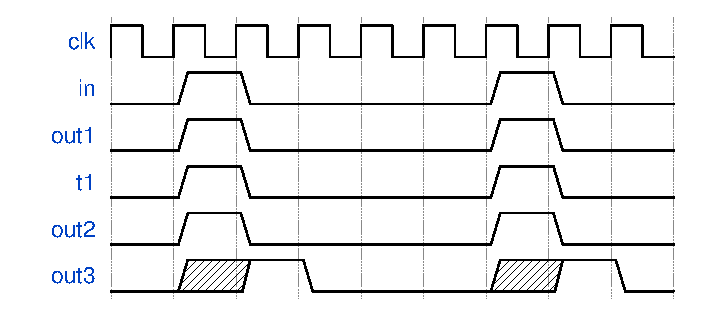
\includegraphics[width=\columnwidth]{figures/wavedrom.eps}%
  \caption{Waveform view showing behavior of RTL design in
  Figure~\ref{figure:equivalence}} 
\label{fig:waveform}
\end{center}
\end{figure}
%
Techniques such as translation validation~\cite{DBLP:conf/tacas/PnueliSS98}  
that check the consistency between an RTL and software is a different problem 
and beyond the scope of this work.
%
%While we do not have a formal proof of equivalence between the Verilog RTL and the 
However, experiments have shown that for 
property verification, valid safety properties are proven to be $k$-inductive for 
the same unwind depth $k$ in the RTL and the software netlist design.  Conversely, 
for unsafe designs, a bug is found in the same unwind depth for both the designs.
 % Equivalence of Hardware and Software
\section{Proposed Verification Tool Flow}
%
\begin{figure}[t]
\centering
\vspace*{0.3cm}
\scalebox{.55}{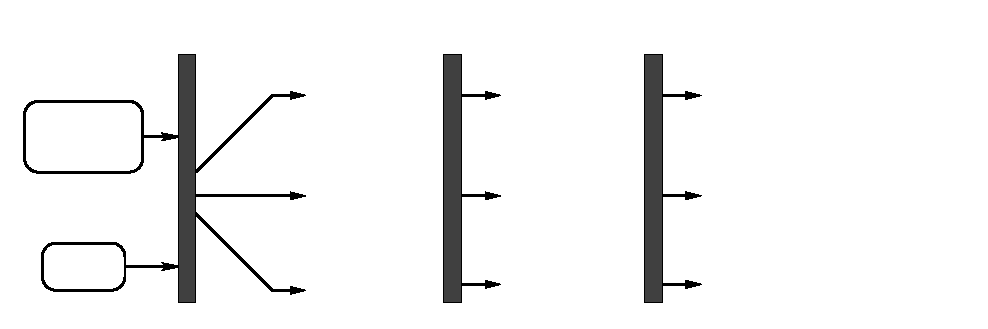
\includegraphics{figures/new_flow_pspdftex.eps}}
\caption{Tool flow for hardware property verification\label{fig:toolflow}}
\end{figure}
%
%===============================================================================
%\subsection{Software Verifiers at the heart of Hardware Verification}
%===============================================================================
%
Figure~\ref{fig:toolflow} gives the tool flow for hardware RTL 
verification using bit-level netlist, word-level netlist and software netlist.  
The bottom flow of Figure~\ref{fig:toolflow} shows the bit-level 
verification flow using ABC.
ABC does not support Verilog, so we use an open-source synthesis tool,
\yosys\footnote{http://www.clifford.at/yosys/} to translate Verilog
RTL to BLIF or AIGER~\footnote{http://fmv.jku.at/aiger/FORMAT-20070427.pdf} 
which is then passed to ABC for verification. 
%Given a design in Verilog RTL, \yosys bit-blasts it into a bit-level netlist 
%along with the property and the resultant netlist is expressed in AIG.  
%The AIG is represented in AIGER format  which is one of the standards 
%andmost prevalant format used by the majority of verification tools.
Whereas, the middle flow of Figure~\ref{fig:toolflow} shows the 
bit/word-level verification using the tool 
EBMC \footnote{www.cprover.org/hardware/ebmc}. 
EBMC supports IEEE 1364.1 Verilog 2005 standards.  EBMC synthesize 
the design in Verilog into a bit-level netlist represented in AIGER or a 
word-level netlist represented in format that resembles the 
SMT-LIB standard. The word-level synthesis flow in EBMC is not mature yet. 
So, we only use the bit-level flow in EBMC. 
%
The top flow of Figure~\ref{fig:toolflow} shows the verification 
of the software netlist designs. 
%verification which translate RTL into software netlist using the tool V2C.  
%
A wide range of representative software 
verification techniques is applied to determine the safety of the
software netlist. In particular, we use $k$-induction~\cite{fmcad2000}
(implemented in the tools CBMC~\cite{cbmc.tacas:2004} and
2LS~\cite{BJKS15}), interpolation
(\cpachecker~\cite{DBLP:conf/cav/BeyerK11}, IMPARA~\cite{impara}), 
Abstract Interpretation (Ast{\'r}ee~\cite{DBLP:conf/esop/CousotCFMMMR05}), 
IC3/PDR (SeaHorn~\cite{DBLP:conf/cav/GurfinkelKKN15}) and Automata-theoretic 
verification (UltimateAutomizer~\cite{DBLP:conf/tacas/HeizmannDGLMSP16}).
%
%===============================================================================
\section{Experimental Results}\label{sec:results}
%===============================================================================
In this section, we report experimental results for \emph{unbounded} safety 
verification of hardware RTL.  Our experimental contributions are two folds.
%
\begin{enumerate}
  \item Compare off-the-shelf formal verification tools for RTL designs by translating  
     them to \emph{bit-level netlist} and \emph{software netlist}.  
    To this end, we compare state-of-the-art hardware model checking tools, such as 
    \emph{ABC 1.01} (winner of HWMCC'15) and 
    \ebmcv~\footnote{\scriptsize{www.cprover.org/hardware/ebmc}}, 
    with various software analyzers from SV-COMP 2016, such as 
    \emph{UltimateAutomizer 3292eade} (winner of SV-COMP'16), 
    \emph{CPAChecker 1.4}, 
    \emph{SeaHorn (revision 07666c810d)}, \emph{2LS 0.3.4}, 
    and a commercial abstract 
    interpretation based tool, \emph{Astr{\'e}e}.  
  
 \item  Compare the performance of unbounded verification algorithms such as $k$-induction, 
    Interpolation, IC3/PDR and Abstraction Interpretation for generating proofs as well as 
    finding complex bugs. 
\end{enumerate}
%
Our experiments were performed on an Intel Xeon machine running at
3.07\,GHz.  We restricted the resources to 5 hours and 32\,GB RAM per
benchmark.  All our benchmarks in Verilog, software netlist in C, 
scripts for running \yosys, ABC, \ebmcv, and other software 
verification tools are available here.~\footnote{\scriptsize{https://github.com/rajdeep87/TCAD-experiments}}
%to a publicly accessible archive website.
%\footnote{\scriptsize{http://www.cprover.org/hardware/tcad/}}
%
%===============================================================================
\subsection{Benchmarks}
%===============================================================================
%
We verified a total of~34 circuits given in Verilog RTL.  Out of 34, 26 
are \emph{safe} benchmarks and 8 are \emph{unsafe}.  The benchmarks in 
our paper are derived from real world hardware benchmark suites, including 
VIS Verilog models, the Texas-97 Benchmark suite, and opencores.org. We synthesize 
each benchmarks into three different netlist formats -- AIGER, SMT-LIB2, ANSI-C.
We classify our benchmarks into two different classes -- data-path intensive
circuits, including Huffman encoder/decoder and a Digital Audio
Input-Output chip (DAIO); and control-intensive designs,
including a non-pipelined 3-stage processor, a Read-Copy-update
mutual exclusion protocol, a FIFO controller, a buffer allocation model,
and an instruction queue controller.   
%
%-------------------------------------------------------------------------------
\subsection{Properties}
%-------------------------------------------------------------------------------
%
The safety properties are specified as System Verilog Assertions.
The SVA properties are translated into C assertions and instrumented 
in the software netlist. 
%
Below, we present few examples of the concurrent assertions in SVA 
and corresponding assertions in the software netlist design.  


Figure~\ref{figure:prop1} and Figure~\ref{figure:prop2} gives 
the SVA property on the left and the corresponding assertions 
in software netlist on the right for the vending machine benchmark 
and Huffman encoder/decoder benchmark, respectively. For the purpose 
of illustration we give partial code fragments for the software 
netlist designs.
%
\begin{example}~\label{safety-prop}
$Assert\_1$: {\em The balance is never negative and never reaches 15.} 
%\vspace{-3mm}
\begin{figure}[htbp]
\centering
\scriptsize
\begin{tabular}{l|l}
\hline
SVA & Assertion (in C)
\\
\hline
\begin{lstlisting}[mathescape=true,language=Verilog]
p1: assert property 
 (@(posedge clk) 
 vending.total[3]==0 && 
 !(vending.total[4:0]==15)); 
\end{lstlisting}
&
\begin{lstlisting}[mathescape=true,language=C]
 assert((((vending.total 
 >> 3) & 0x1) == 0) 
 && !(vending.total 
 & 0x1F == 15));
\end{lstlisting} \\
\hline
\end{tabular}
\caption{Modeling concurrent SVA in software netlist}
\label{figure:prop1}
\end{figure}
%
\end{example}
%
\begin{example}~\label{safety-propnew}
$Assert\_2$: {\em When a new transmission begins, the decoder is ready in the next clock.}
%
\begin{figure}[htbp]
\centering
\scriptsize
\begin{tabular}{l|l}
\hline
SVA & Assertion (in C)
\\
\hline
\begin{lstlisting}[mathescape=true,language=Verilog]
p2: assert property 
 (@(posedge clk) 
 encoder.shiftreg[9:1] 
 == 1 |-> ##1 
 decoder.leaf == 1);
\end{lstlisting}
&
\begin{lstlisting}[mathescape=true,language=C]
 if(((encoder.shiftreg >> 1) 
 & 0x1FF) == 1) {
  // call to top level 
  // module of design
  huffman(clk,addr);  
  assert(decoder.leaf == 1);
 }
\end{lstlisting} \\
\hline
\end{tabular}
\caption{Modeling temporal properties in SVA in software netlist}
\label{figure:prop2}
\end{figure}
\end{example}

%
%-------------------------------------------------------------------------------
\subsection{Discussion}
%-------------------------------------------------------------------------------
We classify the analysis results into two categories -- 1) \emph{precise} tools 
that do not use any abstraction and performs precise reasoning using SAT/SMT solvers 
(in section~\ref{precise}), and \emph{abstraction} based tools that performs 
approximate analysis without using SAT/SMT solvers (in section~\ref{abstraction}). 
%
\subsection{Analysis Using Precise tools}~\label{precise}
%
Figures~\ref{fig:kind}--\ref{fig:hybrid} report the comparison of various unbounded 
verification techniques employed by verification tools at bit-level, word-level, 
and software-level.  The plots in these figures reports the runtimes of~12 
representative circuits which are most difficult to solve out of a total~34 
circuits.  Note that ABC does not implement word-level verification flow, 
so we perform word-level verification using our in-house tool EBMC.
Figures~\ref{fig:kind}--\ref{fig:hybrid} reports the best runtimes 
among the bit-level and word-level hardware verification tools.  
%
We categorize the unbounded approaches into three classes:
\begin{itemize}
\item $k$-induction (Figure~\ref{fig:kind})
\item interpolation (Figure~\ref{fig:impact}), and 
\item PDR together with other hybrid techniques (Figure~\ref{fig:hybrid}).  
\end{itemize}
By hybrid techniques, we refer to predicate
abstraction as implemented in \cpachecker and a combination of
$k$-induction, BMC and abstract interpretation as implemented in
\emph{2LS}~\cite{kiki}.  On the $x$-axis is the analysis time in
seconds and on the $y$-axis we list the benchmarks. The vertical red lines on
the right-hand side of the diagrams show timeouts, out of memory,
inconclusive (unknown) results, errors (crashes), and wrong results
(tool bugs) reported by the tools. The tools can be distinguished 
by the size of the circles as well as by colour. 

\subsection{Analysis using $k$-induction} For safe benchmarks, the results
for bit-level, word-level verifiers and software verifiers are
comparable when the properties are 1-inductive or 2-step inductive.
However, for complex safety properties, ABC and other abstraction
based software analyzers either timeout or took a long time to
terminate.  We investigated the reason for higher verification times
for some safe benchmarks, such as the FIFO controller, the RCU, and Buffer 
Allocation.  We observe that the properties are not $k$-inductive for
sufficiently large values of $k$, e.g.\ (k=1000) and thus tools based
on $k$-induction either timeout or took long time to
compute the inductive invariant sufficient to prove the property. For
the unsafe benchmarks, for example DAIO and the traffic light controller, where
the bugs are manifested only at 64 and 65 clock cycles respectively,
the verification times using ABC and EBMC's $k$-induction engine 
are comparable to \cbmcv and \textsc{2LS}. Figure~\ref{fig:kind} 
reports the time taken by the $k$-induction engine in 
ABC, \ebmcv, \cbmcv and \textsc{2LS}.  We did not report
the time for \cpachecker since the results suggest that 
its $k$-induction engine is not as mature yet. 

\subsection{Analysis using Interpolation} Figure~\ref{fig:impact} reports
the time taken by the interpolation engine in ABC, \textsc{IMPARA}
and \cpachecker. ABC is the fastest in 9 out of 12
designs. However, it timed out on three complex benchmarks, RCU, FIFO
and BufAl, whereas the software interpolation tool, \textsc{IMPARA},
which implements IMPACT algorithm solved three instances out of which
one is the complex FIFO design; yet \textsc{IMPARA} either timed out or
ran out of memory for the remaining designs.  \cpachecker solved
5 out of 12 cases.  None of the interpolation engines was able to
prove RCU and BufAl.

\subsection{Analysis using Hybrid techniques} Figure~\ref{fig:hybrid}
reports the time taken by the IC3/PDR engine in ABC, \emph{SeaHorn}
and other hybrid techniques as implemented in \cpachecker and
\textsc{2LS}. ABC~is the clear winner here; it is the only tool that
proves the FIFO and BufAl benchmarks safe within the given 5h timeout.
\emph{SeaHorn}'s PDR engine solves half of the benchmarks, but
produces false negatives on the other half due to limited support for
bitvectors. \textsc{2LS} successfully solved 8 benchmarks and times 
out on four benchmarks.  \cpachecker's predicate abstraction reliably
solves 7 benchmarks, but timed out on two benchmarks and reports three
wrong results. Note that none of the tools was able to prove RCU.

\Omit{
The bit-level hardware tools performs better than word-level hardware 
verification for our benchmarks.  So, we only report the bit-level results 
obtained using ABC in Figures~\ref{fig:kind}--\ref{fig:hybrid}.
}


%We do not report the results using Astr{\'e}e since it requires manual
%directives for data and control partitioning to avoid imprecision;
%nonetheless it generates many false alarms for safe benchmarks.

%
%%%%%%%%%%%%%%%%%%%%%%%%%%%%%%%%%%%%%%%%%%%%%%%%%%%%%%%%%%%%%%%%%%%%%%%%%%%%%%%%
\begin{figure}
%\scalebox{0.9}{
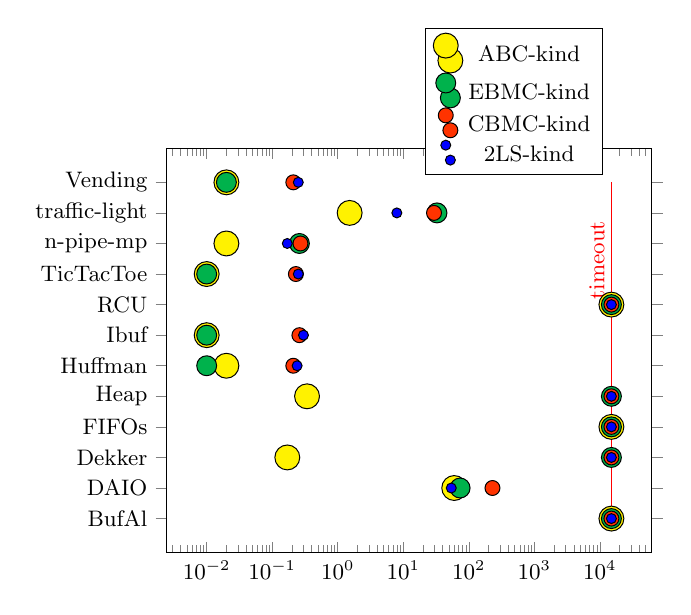
\begin{tikzpicture}[scale=0.9]
\small
\pgfplotstableread{
Benchmark	ABC-kind	EBMC-kind	CBMC-kind	2LS-kind
BufAl	15000	15000	15000	15000
DAIO	59.92	73.62	229.72	54
Dekker	0.17	15000	15000	15000
FIFOs	15000	15000	15000	15000
Heap	0.34	15000	15000	15000
Huffman	0.02	0.01	0.21	0.24
Ibuf	0.01	0.01	0.26	0.3
RCU	15000	15000	15000	15000
TicTacToe	0.01	0.01	0.23	0.25
n-pipe-mp	0.02	0.26	0.27	0.17
traffic-light	1.52	32.67	29.46	7.98
Vending	0.02	0.02	0.21	0.25
}\datatable

\begin{axis}[
    xbar, xmode=log,
    xmin=0,         
    ytick=data,    
    yticklabels from table={\datatable}{Benchmark},  
    legend style={at={(0.9,1.3)}},
]
\addplot [mark size=5pt,only marks, fill=yellow] table [x={ABC-kind}, y expr=\coordindex] {\datatable};    
\addplot [mark size=4pt,only marks, fill=green!70!blue]table [x={EBMC-kind}, y expr=\coordindex] {\datatable};
\addplot [mark size=3pt,only marks, fill=red!80!yellow] table [x={CBMC-kind}, y expr=\coordindex] {\datatable};
\addplot [mark size=2pt,only marks, fill=blue] table [x={2LS-kind}, y expr=\coordindex] {\datatable};
\addplot [red,sharp plot] coordinates{(15000,0) (15000,11)}
          node [left,rotate=90] at (axis cs:9000,10) {timeout};
\legend{{ABC-kind},{EBMC-kind},{CBMC-kind},{2LS-kind}}
\end{axis}
\end{tikzpicture}
%}
\caption{\label{fig:kind}
Comparison of $k$-induction tools
}
\end{figure}
%%%%%%%%%%%%%%%%%%%%%%%%%%%%%%%%%%%%%%%%%%%%%%%%%%%%%%%%%%%%%%%%%%%%%%%%%%%%%%%%

%%%%%%%%%%%%%%%%%%%%%%%%%%%%%%%%%%%%%%%%%%%%%%%%%%%%%%%%%%%%%%%%%%%%%%%%%%%%%%%%
\begin{figure}
%\scalebox{0.9}{
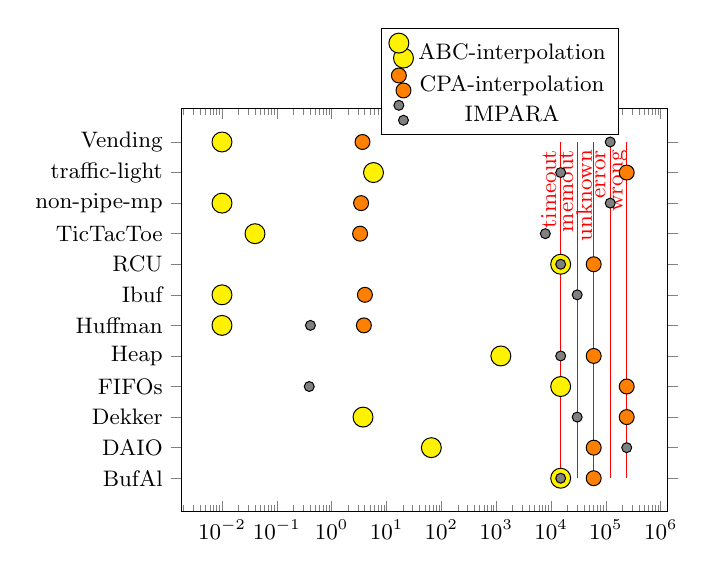
\begin{tikzpicture}[scale=0.9]
\small
\pgfplotstableread{
Benchmark	ABC-interpolation	CPA-interpolation	IMPARA-interpolation
BufAl	15000	60000	15000
DAIO	65.74	60000	240000
Dekker	3.73	240000	30000
FIFOs	15000	240000	0.39
Heap	1215.79	60000	15000
Huffman	0.01	3.87	0.41
Ibuf	0.01	4.04	30000
RCU	15000	60000	15000
TicTacToe	0.04	3.3	7870
non-pipe-mp	0.01	3.44	120000
traffic-light	5.79	240000	15000
Vending	0.01	3.65	120000
}\datatable

\begin{axis}[
    xbar, xmode=log,
    xmin=0,         
    ytick=data,    
    yticklabels from table={\datatable}{Benchmark},  
    legend style={at={(0.9,1.2)}},
]
\addplot [mark size=4pt,only marks, fill=yellow] table [x={ABC-interpolation}, y expr=\coordindex] {\datatable};    
\addplot [mark size=3pt,only marks, fill=orange]table [x={CPA-interpolation}, y expr=\coordindex] {\datatable};
\addplot [mark size=2pt,only marks, fill=gray] table [x={IMPARA-interpolation}, y expr=\coordindex] {\datatable};
\addplot [red,sharp plot] coordinates{(15000,0) (15000,11)}
          node [left,rotate=90] at (axis cs:9000,11) {timeout};
\addplot [red,sharp plot] coordinates{(30000,0) (30000,11)}
          node [left,rotate=90] at (axis cs:19000,11) {memout};
\addplot [red,sharp plot] coordinates{(60000,0) (60000,11)}
          node [left,rotate=90] at (axis cs:40000,11) {unknown};
\addplot [red,sharp plot] coordinates{(120000,0) (120000,11)}
          node [left,rotate=90] at (axis cs:80000,11) {error};
\addplot [red,sharp plot] coordinates{(240000,0) (240000,11)}
          node [left,rotate=90] at (axis cs:180000,11) {wrong};
\legend{{ABC-interpolation},{CPA-interpolation},{IMPARA}}
\end{axis}
\end{tikzpicture}
%}
\caption{\label{fig:impact}
Comparison of interpolation-based tools
}
\end{figure}
%%%%%%%%%%%%%%%%%%%%%%%%%%%%%%%%%%%%%%%%%%%%%%%%%%%%%%%%%%%%%%%%%%%%%%%%%%%%%%%%

%%%%%%%%%%%%%%%%%%%%%%%%%%%%%%%%%%%%%%%%%%%%%%%%%%%%%%%%%%%%%%%%%%%%%%%%%%%%%%%%
\begin{figure}
%\scalebox{0.9}{
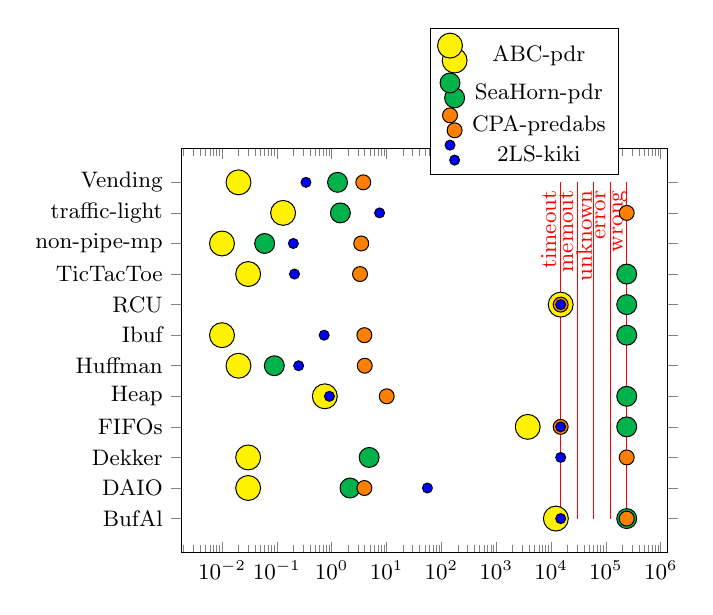
\begin{tikzpicture}[scale=0.9]
\small
\pgfplotstableread{
Benchmark	ABC-pdr	SeaHorn-pdr	CPA-predabs	2LS-kiki
BufAl	12250.5	240000	240000	15000
DAIO	0.03	2.16	3.95	55.72
Dekker	0.03	4.83	240000	15000
FIFOs	3759.75	240000	15000	15000
Heap	0.75	240000	10.09	0.91
Huffman	0.02	0.09	4.01	0.25
Ibuf	0.01	240000	3.95	0.73
RCU	15000	240000	15000	15000
TicTacToe	0.03	240000	3.29	0.21
non-pipe-mp	0.01	0.06	3.46	0.20
traffic-light	0.13	1.44	240000	7.48
Vending	0.02	1.28	3.77	0.34
}\datatable

\begin{axis}[
    xbar, xmode=log,
    xmin=0,         
    ytick=data,    
    yticklabels from table={\datatable}{Benchmark},  
    legend style={at={(0.9,1.3)}},
]
\addplot [mark size=5pt,only marks, fill=yellow] table [x={ABC-pdr}, y expr=\coordindex] {\datatable};    
\addplot [mark size=4pt,only marks, fill=green!70!blue]table [x={SeaHorn-pdr}, y expr=\coordindex] {\datatable};
\addplot [mark size=3pt,only marks, fill=orange] table [x={CPA-predabs}, y expr=\coordindex] {\datatable};
\addplot [mark size=2pt,only marks, fill=blue] table [x={2LS-kiki}, y expr=\coordindex] {\datatable};
\addplot [red,sharp plot] coordinates{(15000,0) (15000,11)}
          node [left,rotate=90] at (axis cs:9000,11) {timeout};
\addplot [red,sharp plot] coordinates{(30000,0) (30000,11)}
          node [left,rotate=90] at (axis cs:19000,11) {memout};
\addplot [red,sharp plot] coordinates{(60000,0) (60000,11)}
          node [left,rotate=90] at (axis cs:40000,11) {unknown};
\addplot [red,sharp plot] coordinates{(120000,0) (120000,11)}
          node [left,rotate=90] at (axis cs:80000,11) {error};
\addplot [red,sharp plot] coordinates{(240000,0) (240000,11)}
          node [left,rotate=90] at (axis cs:180000,11) {wrong};
\legend{{ABC-pdr},{SeaHorn-pdr},{CPA-predabs},{2LS-kiki}}
\end{axis}
\end{tikzpicture}
%}
\caption{\label{fig:hybrid}
Comparison of hybrid techniques
}
\end{figure}
%
%%%%%%%%%%%%%%%%%%% Plot runtimes %%%%%%%%%%%%%%%%%%%%%%%
\begin{figure}[t]
  \centering
  \begin{tikzpicture}[scale=0.60]

\pgfplotscreateplotcyclelist{markstyles}{%
solid, every mark/.append style={solid, fill=white}, mark=square*, mark size=2.5\\%
solid, every mark/.append style={solid, blue}, mark=triangle*,mark size=2.5\\%
solid, every mark/.append style={solid, fill=black}, mark=otimes*,, mark
    size=2.5\\%
}
    
 	%axis
  \begin{axis}[
    width=\linewidth,
    xlabel={Benchmark Number},
    ylabel={Time (seconds)},
    domain = 1:40,
    xmin=1, xmax=40,
    ymin=0, ymax=200,
    %ytick={0,20,...,200},
    xtick={1,5,10,...,40},
    width=15cm, height= 7cm,
    ymode = log,
    %log basis x={2},
    %xticklabel=\pgfmathparse{2^\tick}\pgfmathprintnumber{\pgfmathresult},
    legend pos = north west,
    grid = major,
    major grid style={line width=.2pt,draw=gray!50},
    cycle list name=markstyles
  ]
	
  %plots
  %\addplot table [only marks, y=Time, x=Benchmarks]{plotdata/cbmc.dat};
	%\addlegendentry{CBMC}
  
  \addplot table [only marks, y=Time, x=Benchmarks]{plotdata/abc.dat};
  \addlegendentry{ABC}
  
  \addplot table [only marks, y=Time, x=Benchmarks]{plotdata/astree.dat};
  \addlegendentry{Astr{\'e}e}
	
  \end{axis}  
\end{tikzpicture}
\caption{\label{fig:runtimes}
  Runtime Comparison between ABC and Astr{\'e}e}
\end{figure}

%%%%%%%%%%%%%%%%%%%%%%%%%%%%%%%%%%%%%%%%%%%%%%%%%%%%%%%%%

%
%%%%%%%%%%%%%%%%%%%%%%%%%%%%%%%%%%%%%%%%%%%%%%%%%%%%%%%%%%%%%%%%%%%%%%%%%%%%%%%%
\subsection{Bit-level versus Word-level Analysis}
%%%%%%%%%%%%%%%%%%%%%%%%%%%%%%%%%%%%%%%%%%%%%%%%%%%%%%%%%%%%%%%%%%%%%%%%%%%%%%%%
%
Figure~\ref{fig:solverruntimes} gives the runtime comparison between bit-level 
model checking using SAT solvers and word-level model checking using SMT solvers.  
% 
The SAT (in DIMACS format) and SMT (in SMT-LIB2 format) benchmarks are obtained 
automatically using CBMC from the software netlist design. 
%  
For bit-level results, we report the best runtimes among MiniSAT~\cite{minisat} 
and Lingeling~\cite{lingeling} solvers.  The word-level results are obtained 
using Boolector~\cite{boolector} SMT solver which solved more instances 
than Z3~\cite{z32008} SMT solver. 
%  
The timeout was set to~200 seconds per benchmark.  
%
The runtimes in Figure~\ref{fig:solverruntimes} are obtained for 
a pre-determined unwind bound of~70.  The bit-level engine in CBMC 
wins consistently over the word-level engine, except for the 5~cases 
where Boolector was faster than the bit-level solvers.   
% 
We investigate the reason for the higher runtimes of the 
word-level engine. We observe that the RTL designs used 
for our experiment contains too many bit-slices. 
%, which is also exhibited by the software netlist 
%designs due to the bit-precise translation. 
Hence, pure word-level reasoning performs poorly compared 
to the bit-level analysis since word-level tools also use 
bit blasting for solving such designs. 
%
\subsection{Analysis Using Abstraction based tools}~\label{abstraction}
%
One of the benefits of the proposed tool flow in this paper is that the 
synthesis of RTL to software netlist enables the application of techniques 
such as abstract interpretation. Abstract Interpretation~\cite{Cousot92,CC79} 
is a theory of sound approximation of program semantics based on lattice 
structures. Static analysis using abstract interpretation is widely used 
to verify properties of safety-critical systems. 


Astr{\'e}e~\cite{DBLP:conf/esop/CousotCFMMMR05} is a commercial abstract 
interpretation tool developed by AbsInt~\footnote{https://www.absint.com/}.  
It is primarily used for static analysis of safety-critical softwares 
such as avionics software~\cite{DBLP:journals/corr/abs-cs-0701193}.
Astr{\'e}e employs numeric abstract domains, such as intervals that  
abstract variable values as ranges, as well as relational domains that  
infer linear and non-linear relationships between variables. These abstractions are  
well-suited for programs performing integer and float arithmetic, but  
less so for bit-level Boolean operators, bit-shifts, and bitfields  
packing several values in words.  The non-linear abstract domains in 
Astr{\'e}e such as quadratic and exponential functions are mostly useful 
for aerospace applications~\cite{DBLP:journals/ftpl/BertraneCCFMMR15}.  
Moreover, Astr{\'e}e features BDD-based abstract 
domains~\cite{bdd-domain} that can represent non-convex invariants, 
but they are currently limited to Boolean variables and cannot perform  
bit-blasting on integer variables.  For bit manipulating programs 
generated by \textsc{v2c}, Astr{\'e}e uses default abstract domains 
for integer values such as interval domain, octagon domain, integer 
congruences, integer bitfields, and finite sets (of possible values).


When Astr{\'e}e encounters an \texttt{assert}, it first checks whether 
there are some program states that do not satisfy the assertion, and 
then continues the analysis with only the states that satisfy the assertion. 
Indeed, it assumes that the states that do not satisfy the assertion cause 
the program to stop.  A message such as ``Definite assertion failure" appears 
in case there are no states satisfying the assertion at all, hence, the 
instructions following the assertion are never executed.


Figure~\ref{fig:runtimes} gives the runtime comparison between 
ABC, \textsc{UltimateAutomizer} and Astr{\'e}e.  We choose 
the ABC PDR engine for comparison with abstraction-based software 
analyzers since it performs better than the other verification engines 
and is superior than EBMC on our benchmarks. The tools can be distinguished 
by the shape as well as by colour. 
%
We verified a total of~34 circuits given in Verilog RTL. 
The tools \textsc{UltimateAutomizer} and Astr{\'e}e are fed with the 
software netlist designs generated from the RTL whereas the input to 
ABC is the AIGER representation of the RTL. 
% 
Both \textsc{UltimateAutomizer} and Astr{\'e}e operate 
on an overapproximate abstraction of the concrete program.  
The timeout was set to~200 seconds and memory resources 
were restricted to 32\,GB RAM per benchmark. 
%\todo{reason}


%
ABC proved a total of~30 benchmarks and timed out for 4 benchmarks.  
On the other hand, Astr{\'e}e reported a total of~7 false alarm out of~34 
benchmarks (shown by the blue triangles corresponding to the timeout axis in 
Figure~\ref{fig:runtimes}). However, Astr{\'e}e was faster than ABC on~8 benchmarks (23\% cases).
%
Among these~8 benchmarks,~3 are unsafe for which Astr{\'e}e reported bugs
earlier than ABC. For the remaining~5 benchmarks, ABC timed out in 4 cases, 
whereas Astr{\'e}e proved all~5 benchmarks within the time limit (see the plots 
on the extreme right side of Figure~\ref{fig:runtimes}).  
%
Overall, the runtimes of Astr{\'e}e are very close to ABC for most benchmarks. 
%

We investigate the reason for the false alarms in Astr{\'e}e and observe that 
the bit-manipulating nature of the software netlist prevents Astr{\'e}e from 
inferring the necessary invariants that are required to prove the property 
because these invariants are not expressible by the underlying abstract domains. 

Whereas, \textsc{UltimateAutomizer} timed out in~14 
out of 34 benchmarks. For safe benchmarks that are hard to prove, \textsc{UltimateAutomizer} 
was able to infer the necessary invariants required to prove the property within 
the time limit. 
%which are shown by square boxes between benchmark number 20 to 35. 
%while Astr{\'e}e was too imprecise to prove the property for these benchmarks. 
Whereas, Astr{\'e}e performed better than \textsc{UltimateAutomizer} for all 
unsafe benchmarks.  Astr{\'e}e reported bugs in all 8 unsafe benchmarks within 
the time limit.  We now discuss various ways to improve the precision in
Astr{\'e}e some of which are used for precise verification of the software
netlist designs. 


%%%%%%%%%%%%%%%%%%%%%%%%%%%%%%%%%%%%%%%%%%%%%%%%%%%%%%%%%%%%%%%%%%%%%%%%%%%%%%%%
\begin{figure}[t]
  \centering
  \begin{tikzpicture}[scale=0.60]

\pgfplotscreateplotcyclelist{markstyles}{%
solid, every mark/.append style={solid, fill=white}, mark=square*, mark size=2.5\\%
solid, every mark/.append style={solid, blue}, mark=triangle*,mark size=2.5\\%
solid, every mark/.append style={solid, fill=black}, mark=otimes*,, mark
    size=2.5\\%
}
    
 	%axis
  \begin{axis}[
    width=\linewidth,
    xlabel={Benchmark Number},
    ylabel={Time (seconds)},
    domain = 1:22,
    xmin=1, xmax=22,
    ymin=0, ymax=200,
    %ytick={0,20,...,200},
    xtick={1,4,8,...,22},
    width=15cm, height= 7cm,
    ymode = log,
    %log basis x={2},
    %xticklabel=\pgfmathparse{2^\tick}\pgfmathprintnumber{\pgfmathresult},
    legend pos = north west,
    grid = major,
    major grid style={line width=.2pt,draw=gray!50},
    cycle list name=markstyles
  ]
	
  \addplot table [only marks, y=Time, x=Benchmark]{plotdata/sat.dat};
  \addlegendentry{SAT Solver}
  
  \addplot table [only marks, y=Time, x=Benchmark]{plotdata/smt.dat};
  \addlegendentry{SMT Solver}
  
  \end{axis}  
\end{tikzpicture}
\caption{\label{fig:solverruntimes}
  Runtime comparison between SAT and SMT. Best runtimes among MiniSAT and
  Lingeling is reported in SAT results and the SMT results are reported using
  Boolector solver. The SAT and SMT benchmarks are generated by CBMC for an
  unwind bound of 70.}
\end{figure}

%%%%%%%%%%%%%%%%%%%%%%%%%%%%%%%%%%%%%%%%%%%%%%%%%%%%%%%%%%%%%%%%%%%%%%%%%%%%%%%%
%\subsection{Abstract Interpretation of RTL}
%
%%%%%%%%%%%%%%%%%%%%%%%%%%%%%%%%%%%%%%%%%%%%%%%%%%%%%%%%%%%%%%%%%%%%%%%%%%%%%%%%
%\subsection{Effect of Trace partitioning for Precise analysis in Astr{\'e}e}
%%%%%%%%%%%%%%%%%%%%%%%%%%%%%%%%%%%%%%%%%%%%%%%%%%%%%%%%%%%%%%%%%%%%%%%%%%%%%%%%
%
\subsection{Handling Imprecision in Astr{\'e}e}
%
Given that many abstract domains can only represent convex  
(non-disjunctive) numeric properties, control-flow joins and loop  
widening are a major cause of precision loss.  Astr{\'e}e partially  
alleviates the problem through BDD-based domains and 
trace-partitioning~\cite{DBLP:journals/toplas/RivalM07}
(providing a level of path-sensitivity). 
To prevent scalability issues, these costly techniques are enabled locally, 
through automatic heuristics or user guidance.  That is, a partitioning 
initiated inside a function will be merged over before  
returning from the function, so, it's function-local. Sometimes, a  
longer partitioning is useful, but it is not generated by the  
heuristics (although it can be generated by hand).  While standard 
widening can cause lot of precision loss, Astr{\'e}e 
uses more gradual widening and does not loses all precision at  
once.  We employ widening with thresholds, for instance, and also delay  
the widening (independently on each variable).  


With trace partitioning, Astr{\'e}e automatically insert 
\texttt{\_\_ASTREE\_partition\_control} directives according to a set of 
heuristics.  Astr{\'e}e does not partition ``everything" since this would 
be too expensive in practise. Such a high precision is also normally not 
required for a runtime error analysis. Astr{\'e}e normally start with exisitng 
partitioning heuristics and manually add partitioning directives in places 
where false alarms occur due to a loss of precision resulting from merging 
data-flow information of several control-flow paths (traces).
There are two partitioning strategies in Astr{\'e}e - 
1) control-flow partition and 2) partition over all relevant variable values.
Both can be either specified by hand or using automatic  
partitioning or (more likely) a combination of both. Automatic  
partitioning is simply a fast pre-analysis that inserts  
$\_\_ASTREE\_partition$ directives into the Abstract Syntax Tree.

A classic example of control partitioning is to analyze each branch of a 
control-flow path separately so as to prevent joins at the control-flow merge 
point.  An example of variable partitioning is as follows. Consider a variable 
named \texttt{mode} that can assume values between 1 and 5.  A partitioning directive 
\texttt{\_\_ASTREE\_partition\_begin((mode));} tells Astr{\'e}e to keep all 
five traces for all five possible values of mode apart 
until the next merge point (i.e., the end of a function, a loop, a sub-statement 
or a merge directive). This of course requires Astr{\'e}e to know that mode is 
in the range $[1;5]$.


Although one can theoretically get an arbitrary high precision in Astr{\'e}e by 
partitioning such that all relevant (or in the extreme: possible) execution 
paths are considered separately, but that is not feasible in practice considering 
the analysis times. Hence, the trick is to find the ``right" partitioning that 
is as imprecise as possible, but can still prove the property under verification. 
But this is a challenging task.  
%Astr{\'e}e does not collect data about 
%state-space coverage of variables to help user find a good partitioning. 
However, Astr{\'e}e can show the user any variable range and invariants that 
it has computed.  So, the user can use this information to  
add manually more partitioning and re-run the analysis. What Astr{\'e}e lack  
is a way for this information to be used automatically in partitioning  
strategies during the subsequent analyses.  For our benchmarks, 
%I did not have time to 
we inspect all the invariants inferred by Astr{\'e}e and added the 
necessary partitioning.  A few false alarms in Astr{\'e}e is avoided 
using this strategy.  However, this require manual intervention to 
guide the tool to precisely prove a property of the software netlist model.


%Hence, some amount of domain knowledge is required to try different partitioning 
%strategies that might enable the analysis to prove the properties under verification. 
%For our experiments, we ran the analysis using the existing heuristics and manual 
%partitioning on data as well as control that target automatically-generated 
%software netlist obtained from V2C and 
%was sufficient to precisely prove the properties. 


\Omit{
There can be various sources of imprecision in abstract 
interpretation.  Few common sources of imprecision may occur due to   
\emph{control-flow join}, \emph{loop widening} or use of \emph{imprecise abstract domain}.  
We analyzed the structure of software netlist models to detect the potential sources of 
imprecision that may occur during the analysis using Astr{\'e}e.  Recall that the software 
netlist model retains the control structure of the input RTL design.  Hence, if the original 
RTL has loops or conditional branches inside a module, a software netlist also preserves the 
similar control structure.   
}

\subsection{Soundness of Astr{\'e}e}
%
Astr{\'e}e is sound, that is, it does not miss any genuine error. 
However, it errs for the safe benchmarks, sometimes too much. Hence, Astr{\'e}e 
may report more false positives than other tools. However, Astr{\'e}e 
found genuine bugs in all 8 unsafe benchmarks.
%(doing otherwise would be a bug in Astrée). 
In general, a sound tool is useful for validation, less so for 
bug-finding.


\Omit{Standard Static Analysis is Imprecise, but can we do better than bit
blasting ? 

\subsection{Idea} Partition the traces so that we can prove correctness for each partition.
\subsection{Solution} To be effecient, we want partitions that are just precise
enough. 
}
\Omit{Best HW runtime versus Best Software runtimes}

\subsection{Summary of the results} 
%
We summarize the results obtained from the precise and abstraction-based 
software analyzers for verifying the software netlist designs.


%%%%%%%%%% CAV Reviews %%%%%%%%%%%%%%
A fundamental difference betwen the hardware and software designs is that 
hardware designs tend to use bit-slices to model various functionality 
including power, performance logic.  The software netlist models the 
bit-level hardware logic using combinations of bit-wise operations, 
such as shift, bitwise-AND, bit-masking etc.  
%
This often makes the software netlist designs hard to analyze 
%operators which make it harder for word-level tools to reason about these designs, 
as looking at shift and AND operators, in general, would be difficult 
to reverse them to their original bit-slice intention.
%
A common solution is to partition the original word to adapt to the user 
defined bit-slices.  However, this approach would not be feasible since 
the software netlist design is modeled in the C language, which support word-level 
variables of fixed width (e.g. 32 bits or 64 bits). So this is inherently 
a problem that is not addressed by software analyzers.

\subsection{Analysis using Precise SAT/SMT based Software Analyzers}
%
Though the invariant inference techniques employed by precise software 
analyzers such as \cpachecker and 2LS have never
been optimized for hardware analysis, the results in this chapter 
show that these tools are within one order of magnitude compared to
bit-level hardware model checkers for detecting bugs as well as 
proving safety of some of the software netlist designs.  However, 
running SAT/SMT based software analyzers on the software netlist 
designs exhibits many 
%tool bugs (marked as ``wrong'' in Figure).
%We investigated the reason for large number of 
timeouts, wrong results and errors.  We observed that software netlists 
heavily use bit-level operations and thus bit-precise reasoning ability 
is necessary to precisely reason about these designs.  But, bit-level 
operations are less prevalent in conventional software and hence less 
tested in software analysis tools.  We reported the tool bugs to the 
authors of these tools.


\subsection{Analysis using Abstraction based Software Analyzers}
%
The abstraction-based software analyzers such as Ultimate Automizer and Astr{\'e}e 
performed better than the SAT/SMT-based software analysis tools.  Though 
Astr{\'e}e require manual intervention to select the right set of partitions 
of program traces in order to do precise analysis, the verification runtimes 
of Astr{\'e}e are comparable to ABC for most of the benchmarks.  However, 
Astr{\'e}e often uses numerical abstractions, which are likely to lose 
important bit-precise information.  
%
As a consequence, many inductive invariants required by the bit-manipulating 
benchmarks cannot be represented, and so not inferred, using current abstractions 
in Astr{\'e}e.  An abstract domain for this purpose must keep 
precise relations between the bits of an integer (possibly some 
form of BDD on the bits of the variable).  Astr{\'e}e has already been 
refined for avionics and space software by adding few domain-specific 
abstract domains which were very effective in removing some classes of 
false alarms~\cite{DBLP:journals/ftpl/BertraneCCFMMR15}.  We thus believe 
that there is scope here for new abstract domains targeting hardware 
designs while still remaining within the scope of the traditional abstract 
interpretation. 
%
%that implement abstract interpretation using
%abstract domains developed specifically for this task, e.g.~by
%applying abstract conflict driven learning~\cite{dhk2013-popl}.  
%-------------------------------------------------------------------------------
\subsection{Limitations of the Result}
%-------------------------------------------------------------------------------
% 
We discuss some of the limitations of the results presented in this paper.  
%Firstly, the publicly available Verilog RTL designs often lack requirement 
%specifications.  Hence, it is difficult to write meaningful 
%properties for verifying these designs.  
Firstly, the benchmarks used in this paper are limited to block-level 
designs which are obtained from publicly available repository. 
% 
Secondly, most of the properties that we verified are either global properties 
or temporal bounded properties, that is, they are either of the form 
$G(x)$, where $x$ must be \emph{true} globally or is of the form 
$x \mapsto \#\#[1:3] y$, where an event $y$ is asserted between 1st and 
3rd timeframe after the event $x$ has happened.  We did not verify 
properties with \emph{eventual} or \emph{release} operators. 
%  
Thirdly, the proposed approach is only used for the verification of the 
single-clock RTL designs that does not employ clock-gating or power-gating 
techniques~\cite{lowpower}.  
Hence, abstracting the RTL clock in the software netlist does not have any 
impact on the verification outcome in our experiments.  
%  
However, designs that exhibit clock-gating or power-gating techniques or 
designs that contain multiple clocks may be non-trivial to translate and 
may require modeling the behavior of clock explicitly in the software netlist. 
%
\Omit{
Thirdly, our experiments compare formal verification of RTL designs by 
translating them to bit-level netlist and software netlist.  
%
For some of the designs (8 out of 34), we used the word-level synthesis 
flow in EBMC.  
We observed that the result of the word-level verification in EBMC 
using Z3 theorem prover is absolutely the same as the bit-level 
verification for these 8 benchmarks. The translation of word-level 
netlist to SMT-LIB2 format is not mature yet in EBMC (we could not 
translate the remaining 26 benchmarks), so we could not give the 
word-level verification results in this paper. Furthermore, 
ABC does not fully support word-level verification.  
}
   
\section{Related Work}~\label{related_work}
%
%%%%%%%%%%%%%%%%%%%%%%%%%%%%%%%%%%%%%%%%%%%%%%
%      Bit-level Verification Literature
%%%%%%%%%%%%%%%%%%%%%%%%%%%%%%%%%%%%%%%%%%%%%%

%%%%%%%%%%%%%%%%%%%%%%%%%%%%%%%%%%%%%%%%%%%%%%
%     Word-level Verification Literature
%%%%%%%%%%%%%%%%%%%%%%%%%%%%%%%%%%%%%%%%%%%%%%

%%%%%%%%%%%%%%%%%%%%%%%%%%%%%%%%%%%%%%%%%%%%%%
%      Software verification Literature
%%%%%%%%%%%%%%%%%%%%%%%%%%%%%%%%%%%%%%%%%%%%%%

The technology transfer between the hardware and software verification community 
over the past two decades have demonstrated significant drive in development of 
new verification algorithms in either field. 
% 
In 1986, Clarke et al.~\cite{clarke86} proposed model checking for finite state 
concurrent systems. Later, McMillan et. al.~\cite{mcmillan96} introduced symbolic 
model checking in 1996.  Biere et al.~\cite{tacas99} introduced symbolic model 
checking without BDDs in 1999.
%
Graf et al.~\cite{cav97} proposed a technique based on predicate abstraction.
Later, Clarke et. al.~\cite{cav2000} used Counterexample guided Abstraction Refinement 
(CEGAR) in SMV tool for verifying Fujitsu IP core.  
Kroening et. al.~\cite{DBLP:conf/tacas/JainKSC07} used CEGAR to 
verify hardware designs written in Verilog RTL.  Subsequently, predicate 
abstraction is used for verifying device drivers in C program by Ball et al.~\cite{pldi01}.  
This lead to the SLAM project by Ball et. al.~\cite{popl02} in 2002.
%
In 2000, St$\mathring{\text{a}}$lmarck et al.~\cite{fmcad2000} introduced a technique 
to check safety properties using Induction and SAT solver.  Subsequnetly, induction 
based approaches are used for automatic analysis of scratch-pad memory code for heterogeneous
multicore processors by Donaldson et. al.~\cite{tacas10}, 2010 and for software 
verification using k-induction by Donaldson et al.~\cite{sas2011} in 2011.
% 
In 2003, McMillan et al.~\cite{cav03} introduced Interpolation and SAT-based model 
checking for verifying commercial microprocessor. Subsequently, Intrpolation is used 
for software verification by McMillan et. al.~\cite{cav06} in 2006 and by 
Kroening et al.~\cite{DBLP:conf/cav/KroeningW11}, in 2011.
%
In 2007, Bradley et. al.~\cite{fmcad07} introduced safety checking by inductive 
generalizations of counterexample to induction, a technique commonly known 
as IC3. Subsequnetly, IC3 is used for software model checking by 
Cimatti et al.~\cite{cav12ic3} in 2012.
%
Thus, techniques like predicate abstraction, 
IC3 or Property Directed Reachability (PDR), $k$-induction, and 
interpolation-based approaches have all made their way from the hardware 
to the software domain; but path-wise symbolic execution and abstract 
interpretation have been primarily used for software verification.
%
A survey of bounded and unbounded SAT-based hardware model checking techniques 
is presented in~\cite{DBLP:conf/charme/AmlaDKKM05}.
%

\Omit{
A survey of bounded and unbounded SAT-based hardware model checking techniques 
is presented in~\cite{charme05}.
Table~\ref{timeline} provides a summary of technology transfer between the 
hardware verification community and software verification community over the past 
two decades.  The table provides the reference to the very first technique proposed 
in the literature in either community but there are subsequent works that
follows up from these.  For example, techniques like predicate abstraction, 
IC3 or Property Directed Reachability (PDR), $k$-induction, and 
interpolation-based approaches have all made their way from the hardware 
to the software domain; but path-wise symbolic execution and abstract 
interpretation have been primarily used for software verification.
%
\begin{table}[]
\centering
\scriptsize
\caption{Technology transfer between the Hardware and Software Verification Community}
\label{timeline}
\begin{tabular}{p{0.2\textwidth}|p{0.2\textwidth}}
\toprule
  Hardware Verification & Software Verification \\
  \midrule
  \begin{itemize}
  \item Symbolic Model Checking without BDDs 
    by Biere et. al.~\cite{tacas99}, 1999
\end{itemize}
 & 
 \begin{itemize}
  \item Model Checking for finite state concurrent systems by Clarke et
    al.~\cite{clarke86}, 1986
  \item Symbolic Model Checking by McMillan et. al.~\cite{mcmillan96}, 1996
\end{itemize} \\ \hline

 \begin{itemize}
 \item Predicate Abstraction by Graf et. al.~\cite{cav97}, 1997
 \item CEGAR in SMV for verifying Fujitsu IP core by Clarke et.
   al.~\cite{cav2000}, 2000 
 %\item CEGAR for Verilog by Kroening et. al.~\cite{tacas07}, 2007
 \end{itemize}
  &
  \begin{itemize}
    \item Predicate Abstraction for C program by Ball et. al.~\cite{pldi01},
      2001
    \item SLAM project by Ball et. al.~\cite{popl02}, 2002
  \end{itemize} \\ \hline
 
  \begin{itemize}
    \item Checking safety properties using Induction and SAT solver by
      St$\mathring{\text{a}}$lmarck et. al.~\cite{fmcad2000}, 2000
   \end{itemize}
   & 
   \begin{itemize}
     \item Automatic analysis of scratch-pad memory code for heterogeneous
       multicore processors by Donaldson et. al.~\cite{tacas10}, 2010
     \item Software verification using k-induction by Donaldson et.
       al.~\cite{sas2011}, 2011
   \end{itemize} \\ \hline
   
   \begin{itemize}
     \item Interpolation and SAT-based model checking for verifying commercial
       microprocessor by McMillan et. al.~\cite{cav03}, 2003
   \end{itemize}
   & 
   \begin{itemize}
     \item Lazy abstraction with interpolants by McMillan et. al.~\cite{cav06}, 2006
     \item Interpolation based software verification with Wolverine by Kroening
       et. al.~\cite{cav11}, 2011
   \end{itemize} \\ \hline
   
   \begin{itemize}
     \item Checking safety by inductive generalizations of counterexample to
       induction by Bradley et. al.~\cite{fmcad07}, 2007
   \end{itemize}
   &
   \begin{itemize}
    \item Software Model Checking via IC3 by Cimatti et. al.~\cite{cav12ic3}, 2012
   \end{itemize} \\ \hline
\bottomrule
\end{tabular}
\end{table}
%
}

\section{Conclusions and Prospects}\label{sec:concl}
%
Demand for more scalable verification tools is ever growing.  In this paper,
we present an alternative solution for verifying hardware, at the heart of
which is a verifier for software.  To this end, we present a technique to 
synthesize a software netlist from Verilog RTL.  We then use state-of-the-art
software verification tools to verify these software netlist models.  Our 
experimental results present a detailed comparison of various unbounded 
verification algorithms at bit-level, word-level and software level.  Our proposed 
hardware verification flow enables seamless adoption of any advances in software 
verification technology to RTL verification.  We observe that bit-level operations 
are less prevelant in conventional software and hence software analyzers are not 
optimized to reason about bit manipulating software programs.  However, most software 
tools are able to successfully verify RTL circuits and the performance of these tools 
are within an order of magnitude compared to bit-level hardware tools.  Existing abstract 
domains used in abstraction based software tools are insufficient for precise reasoning 
of software netlist models.  This can be addressed by either developing heuristics 
more adapted to the code generated by v2c, or manually annotating the generated code 
to improve the precision of the analysis. In this paper, we follow the later approach 
to obtain the desired results. 
    % Conclusions

% ---------------------------------------------------------------------
% Un-numbered section of acknowledgments
% ---------------------------------------------------------------------

\section*{Acknowledgments}

% ---------------------------------------------------------------------
% Bibliography
% ---------------------------------------------------------------------

\bibliographystyle{IEEEtran}
\bibliography{biblio}

% ---------------------------------------------------------------------
% Biographies of authors.
% ---------------------------------------------------------------------

% \begin{IEEEbiography}{Rajdeep Mukherjee}
% \end{IEEEbiography}

% \begin{IEEEbiography}{Peter Schrammel}
% \end{IEEEbiography}

% \begin{IEEEbiography}{Tom Melham}
% \end{IEEEbiography}

% \begin{IEEEbiography}{Daniel Kroening}
% \end{IEEEbiography}

% \begin{IEEEbiography}{Michael Tautschnig}
% \end{IEEEbiography}

\end{document}


